\documentclass[a4paper,12pt]{article}

% Pacchetti utili
\usepackage[italian]{babel}
\usepackage[T1]{fontenc}
\usepackage[utf8]{inputenc}
\usepackage{lmodern}
\usepackage{geometry}
\usepackage{setspace}
\usepackage{graphicx}
\usepackage{titling}
\usepackage{hyperref}
\usepackage{booktabs}
\usepackage{amsmath, amssymb}
\usepackage[most]{tcolorbox}
\usepackage{tikz}
\usetikzlibrary{positioning, arrows.meta, calc}

\geometry{margin=2.5cm}
\onehalfspacing

\begin{document}
	
	\begin{titlepage}
		\centering
		
		% Intestazione Università
		{\scshape\LARGE Università di Pisa \par}
		\vspace{0.5cm}
		
		% Titolo corso
		{\Huge\bfseries Calcolo Numerico \par}
		\vspace{0.5cm}
		{\Large Anno Accademico 2025--2026 \par}
		
		\vfill
		
		% Autore
		{\Large\textbf{Pietro Bacigalupi} \par}
		\vspace{0.5cm}
		
		\vfill
		
		% Data
		{\large \today\par}
		
	\end{titlepage}
	
	\tableofcontents
	\newpage
	
	\section{Teoria degli Errori}
	
	\subsection{Rappresentazione in Virgola Mobile}
	
	Fissata una base $\beta > 1$, con $\beta \in \mathbb{N}$, un numero reale $x$ può essere rappresentato nella forma:
	
	\begin{equation}
		x = \mathrm{segno}(x) \cdot \beta^{e} \cdot \sum_{i=1}^{\infty} \alpha_i \, \beta^{-i}
	\end{equation}
	
	dove:
	
	\begin{itemize}
		\item $\beta$ è la base della rappresentazione;
		\item $e \in \mathbb{Z}$ è l'esponente;
		\item $\alpha_i$ sono le cifre della mantissa, tali che
	\end{itemize}
	
	\begin{equation}
		0 \le \alpha_i \le \beta - 1
	\end{equation}
	
	e
	
	\[
	\mathrm{segno}(x) =
	\begin{cases}
		+1 & \text{se } x > 0 \\
		-1 & \text{se } x < 0
	\end{cases}
	\]
	
	\begin{tcolorbox}[title=Attenzione, colback=white]
		La rappresentazione così non è unica, ad esempio: $3{,}14 = 0{,}0314 \cdot 10^{2}$.
	\end{tcolorbox}
	
	\subsection{Teorema di Rappresentazione}
	Data $\beta > 1 \in \mathbb{N}$, $x \in \mathbb{R} \neq 0$ allora $\exists!$ rappresentazione di $x$ in base $\beta :$
	
	\begin{enumerate}
		\item $\alpha_1 \neq 0$
		\item $\nexists K \in \mathbb{N} : \alpha_j = \beta-1 \forall j>k$
	\end{enumerate}
	
	L'unica rappresentazione che verifica il teorema si dice \textbf{Rappresentazione in virgola mobile normalizzata}.
	Dove $\sum_{i=1}^{\infty} \alpha_i \, \beta^{-i}$ si dice \textbf{Mantissa} di $x \in \mathbb{R}$ e vale sempre che $ \beta^{-1} < \sum_{i=1}^{\infty} \alpha_i \, \beta^{-i} < 1$
	
	\begin{tcolorbox}[title=Esempio]
		La $(1)$ esclude rappresentazioni con primo numero decimale uguale a 0:
		\begin{itemize}
			\item $0,\mathbf{0}123 \cdot 10^{3}$ Non va bene
			\item $1230,\mathbf{0} \cdot 10^{0}$ Non va bene
			\item $0,123 \cdot 10^{5}$ Va bene
		\end{itemize}
		La $(2)$ esclude numeri in periodici con 9 finali (Esempio $1,4\overline{9}$, in base 10)
 	\end{tcolorbox}
 	
 	\subsection{Numeri di Macchina}
 	
 	\paragraph{Problema}: abbiamo $\inf$ cifre, ne possiamo tenere in considerazione solo un numero finito. Come facciamo? Tronchiamo la mantissa e limitiamo l'esponente.
 	
 	\paragraph{Definizione}: Dati, $\beta$, $m$, $L$, $U$, $\beta>1$, $L \leq u$ e $m>0$ definiamo $\textbf{Insieme dei numeri di macchina}$ la funzione
		\[
		F(\beta,m,L,U) =
		\left\{
		x \in \mathbb{R}
		\;\middle|\;
		x = \mathrm{segno}(x)\,\beta^{e}
		\sum_{i=1}^{m} \alpha_i \beta^{-i},
		\;
		L \le e \le U,
		\;
		\alpha_i \in \{0,1,\dots,\beta-1\},
		\;
		\alpha_1 \neq 0
		\right\} \cup \left\{0\right\}
		\]
		
		I numeri di macchina sono un sottoinsieme dei numeri reali esattamente rappresentabili da un software 
		
		\paragraph{Esempio} $\beta = 2$ $m = 3$ $L = -1$ $U = 3$
		Ci sono un numero costante di elementi in $\left[\beta^{e-1}, \beta^{e}\right)$ e sono equispaziati.\newline
		Stiamo studiando quindi i \textbf{numeri macchina di base 2 con 3 cifre di mantissa} ed esponente da -1 a 3 \newline
		Sono equispaziati in \textbf{scala logaritmica} negli intervalli
		\begin{equation*}
			\left[2^{i}, 2^{i+1}\right)
		\end{equation*}
		quindi:
		\begin{enumerate}
			\item $\left[2^{-1}, 2^{0}\right) =  \left[1/2, 1\right]$
			\item $\left[2^{0}, 2^{1}\right) =  \left[1, 2\right]$
			\item $\left[2^{1}, 2^{2}\right) =  \left[2, 4\right]$
			\item $\left[2^{2}, 2^{3}\right) =  \left[4, 8\right]$
		\end{enumerate}
		\begin{tcolorbox} [title=Osservazione]
			Minimo Rappresentabile:
			\begin{equation*}
				\mathbf{\beta^{L} \cdot \alpha_1 \cdot \beta^{-1} = \beta^{L-1}} \text{ dato che } \alpha_1 = 1
			\end{equation*}
			
			Massimo Rappresentabile:
			\begin{equation*}
				\beta^{U}\cdot\left(\beta-1\right)\sum_{j=1}^{m}\beta^{-j} = \beta^{U}\cdot\left(\beta-1\right)\left(\frac{1-\beta^{-m-1}}{1-\beta^{-1}}-1\right)
				= \beta^{U}\left(1-\beta^{-m}\right)
			\end{equation*}
			
			Quanti sono i numeri macchina rappresentabili:
			
			\[
			\underbrace{2}_{\text{segno}}
			\quad
			\underbrace{(U - L + 1)}_{\text{esponente}}
			\quad
			\underbrace{\left(\beta^{m} - \beta^{m-1}\right)}_{\text{mantissa}}
			\quad
			\underbrace{+1}_{\{0\}}
			\]
		\end{tcolorbox}
		
	\subsection{Arrotondamento nelle macchine}
	\begin{table}[h!]
		\centering
		\begin{tabular}{l c c c c c c c}
			\toprule
			Formato & $\beta$ & $m$ & $L$ & $U$ & Byte & $\varepsilon (precisione)$ & $|F|$ \\
			\midrule
			Double & 2 & 53 & -1021 & 1024 & 8 & $2^{-52}$ & $2(2046)(2^{53}-2^{52})+1$ \\
			Single & 2 & 24 & -124  & 128  & 4 & $2^{-23}$ & $2(253)(2^{24}-2^{23})+1$ \\
			\bottomrule
		\end{tabular}
		\caption{Parametri IEEE 754 in virgola mobile}
	\end{table}
	\paragraph{Osservazione}
	Dato $x \in \mathbb{R}$, in generale $x \notin F(\beta,m,L,U)$.
	Si distinguono tre casi:
	
	\begin{enumerate}
		\item Se $|x| > \beta^{U}(1-\beta^{-m})$ si ha \textbf{overflow}.
		
		\item Se $0 < |x| < \beta^{L-1}$ si ha \textbf{underflow}.
		
		\item Se
		\[
		\beta^{L-1} \le |x| \le \beta^{U}(1-\beta^{-m}),
		\]
		il numero è rappresentabile in ordine di grandezza ma può richiedere
		\textbf{arrotondamento}.
	\end{enumerate}
	
	\paragraph{Definizione}
	Si definisce \textbf{funzione di arrotondamento} una funzione
	
	\[
	\mathrm{RD} : \mathbb{R} \longrightarrow F(\beta,m,L,U)
	\]
	
	che ad ogni numero reale $x$ associa un numero macchina
	$\mathrm{RD}(x)$ appartenente all'insieme $F(\beta,m,L,U)$.	
	
	Le scelte più comuni sono:
	\begin{enumerate}
		\item \textbf{Troncamento}: $TR(x) = \lfloor x \rfloor \forall x$
		\item \textbf{Round-UP}: $UP(x) = \lceil x \rceil \forall x$
		\item \textbf{Round-To-Nearest}: 
		\[
		\mathrm{RN(x)} = 
		\begin{cases}
			\lfloor x \rfloor \textrm{ se } \alpha_{m+1} < \frac{\beta}{2} \\
			\lceil x \rceil \textrm{ se } \alpha_{m+1} \geq \frac{\beta}{2}
		\end{cases}
		\]
	\end{enumerate}
	Quella usata dai calcolatori, che useremo noi, è la \textbf{(3)}
	
	\paragraph{Definizione}
	
	Sia $x \in \mathbb{R}$ e sia $\mathrm{RN}(x)$ il numero macchina ottenuto
	mediante arrotondamento al più vicino (round-to-nearest).
	
	\medskip
	
	Si definisce \textbf{errore assoluto di arrotondamento} la quantità
	
	\[
	\delta(x) = x - \mathrm{RN}(x).
	\]
	
	Si definisce \textbf{errore relativo di arrotondamento} la quantità
	
	\[
	\varepsilon(x) = \frac{\delta(x)}{x},
	\qquad x \neq 0.
	\]
	
	\medskip
	
	Nel caso di arrotondamento al più vicino vale la stima
	
	\[
	|\delta(x)| \le \frac{1}{2}\,\beta^{e-m}.
	\]
	
	Poiché $|x| \ge \beta^{e-1}$, si ottiene
	
	\[
	|\varepsilon(x)|
	= \frac{|\delta(x)|}{|x|}
	\le
	\frac{\frac{1}{2}\beta^{e-m}}{\beta^{e-1}}
	=
	\frac{1}{2}\beta^{1-m}.
	\]
	
	Si osserva che il termine finale non dipende da $x$.
	
	\medskip
	
	La quantità
	
	\[
	u = \frac{1}{2}\beta^{1-m}
	\]
	
	è detta \textbf{precisione di macchina} (o \emph{unit roundoff}).
	In doppia precisione (IEEE 754):
	\[
	u = 2^{-53} \approx 1.11 \times 10^{-16}.
	\]
	
	\subsection{Errore nel calcolo di funzione} 
	Le operazioni di macchina sono 4 e sono $\otimes \oplus \ominus \oslash$ dove
	\begin{itemize}
		\item $x \oplus y = RN(x+y)$
		\item $x \ominus y = RN(x-y)$
		\item $x \otimes y = RN(x \cdot y)$
		\item $x \oslash y = RN(x \div y)$
	\end{itemize} 
	Non è valida la proprietà associativa e distributiva
	\subsubsection{Analisi dell'Errore nel Calcolo di Funzioni}
	
	Sia $f: \mathbb{R}^m \to \mathbb{R}$ una funzione matematica che vogliamo valutare.
	Si vuole calcolare il valore $f(p_0)$, dove il punto di partenza è un vettore di $m$ componenti:
	\[
	p_0 = (x_1^{(0)}, x_2^{(0)}, \dots, x_m^{(0)}) \in \mathbb{R}^m
	\]
	
	\paragraph{Fonti dell'errore:}
	Nel passaggio dalla teoria alla pratica, incontriamo tre ostacoli principali:
	
	\begin{enumerate}
		\item \textbf{Approssimazione della funzione}: La funzione teorica $f$ viene sostituita da una funzione $\tilde{f}$ che il calcolatore sa gestire (ovvero che usa solo operazioni elementari). 
		\textit{Esempio: calcolare $e^x$ usando solo i primi termini dello sviluppo di Taylor.}
		
		\item \textbf{Algoritmizzazione}: La funzione $\tilde{f}$ viene tradotta in un algoritmo $\tilde{f}_a$. Qui entrano in gioco le operazioni di macchina $\oplus, \ominus, \otimes, \oslash$, ognuna delle quali introduce un errore di arrotondamento.
		
		\item \textbf{Arrotondamento dei dati}: Il punto $p_0$ originale spesso non è rappresentabile esattamente in memoria (pensa a $\pi$ o a numeri con troppe cifre). Viene quindi sostituito dal numero di macchina più vicino: $p_1 = \mathrm{RN}(p_0)$.
	\end{enumerate}
	
	\begin{tcolorbox}[colback=yellow!5!white, colframe=yellow!50!black]
		\textbf{Conclusione}: Il nostro obiettivo sarebbe ottenere $f(p_0)$, ma ciò che il computer ci restituisce effettivamente è $\tilde{f}_a(p_1)$.
	\end{tcolorbox}
	\paragraph{Esempio: Calcolo di $e^{\pi}$}
	
	Vogliamo calcolare il valore della funzione $f(x) = e^x$ nel punto $p_0 = \pi$.
	
	\begin{enumerate}
		\item \textbf{Approssimazione matematica}: Poiché il calcolatore non può calcolare la funzione esponenziale esatta, usiamo uno sviluppo di Taylor troncato al secondo ordine:
		\[ f(x) \approx 1 + x + \frac{x^2}{2} =: \tilde{f}(x) \]
		
		\item \textbf{Arrotondamento dell'input}: Il numero $\pi$ ha infinite cifre. Lo arrotondiamo a un numero di macchina $p_1$ (nell'esempio con 5 cifre):
		\[ p_1 = RN(\pi) = 3.1415 \]
		
		\item \textbf{Esecuzione dell'algoritmo}: Implementiamo la formula usando solo operazioni di macchina. L'ordine scelto definisce l'algoritmo $\tilde{f}_a(p_1)$:
		\[ \tilde{f}_a(p_1) = 1 \oplus \left( p_1 \oplus \left( (p_1 \otimes p_1) \oslash 2 \right) \right) \]
	\end{enumerate}
	\paragraph{Grafo computazionale:}
	L'algoritmo sopra descritto può essere visualizzato tramite il seguente schema di flusso:
	
	\begin{center}
		\begin{tikzpicture}[
			node distance=1.5cm and 2cm,
			op/.style={circle, draw, minimum size=1cm, inner sep=0pt},
			thick,
			>={Stealth[length=2mm]}
			]
			% Nodi di input (x)
			\node[op] (x1) {$x$};
			\node[op] (x2) [below=0.6cm of x1] {$x$};
			\node[op] (x3) [below=1.5cm of x2] {$x$};
			
			% Nodo x^2
			\node[op] (sq) [right=of x1, yshift=-0.5cm] {$x^2$};
			\draw[->] (x1) -- (sq) node[midway, above] {$\otimes$};
			\draw[->] (x2) -| (sq) node[pos=0.8, right] {$\otimes$};
			
			% Nodo x^2/2
			\node[op] (div) [right=of sq] {$\frac{x^2}{2}$};
			\draw[->] (sq) -- (div) node[midway, above] {$\oslash$};
			
			% Nodo x^2/2 + x
			\node[op] (add1) [right=of div] {$\frac{x^2}{2} + x$};
			\draw[->] (div) -- (add1) node[midway, above] {$\oplus$};
			\draw[->] (x3) -| (add1) node[pos=0.8, right] {$\oplus$};
			
			% Nodo finale
			\node[op] (final) [right=of add1] {\footnotesize $1 + x + \frac{x^2}{2}$};
			\draw[->] (add1) -- (final) node[midway, above] {$\oplus$};
			
		\end{tikzpicture}
	\end{center}
	\paragraph{Analisi e Spiegazione del Grafo Computazionale}
	
	Il grafo sopra riportato rappresenta la struttura logica e sequenziale dell'algoritmo $\tilde{f}_a(p_1)$. In analisi numerica, questo schema è fondamentale per visualizzare come l'errore si genera e si propaga attraverso i calcoli.
	
	\begin{itemize}
		\item \textbf{Nodi di Input (Sorgenti)}: I cerchi a sinistra contenenti $x$ rappresentano il numero di macchina $p_1 = RN(\pi)$. Nel grafo, lo stesso valore $x$ viene "pescato" tre volte dalla memoria per alimentare i diversi rami del calcolo.
		
		\item \textbf{Nodi Operatori (Cerchi con $\otimes, \oslash, \oplus$)}: Ogni cerchio che contiene un simbolo operativo rappresenta un'operazione di macchina. 
		\begin{itemize}
			\item Il primo nodo esegue $x \otimes x$, producendo il risultato parziale $x^2$. 
			\item Il secondo nodo riceve $x^2$ e lo divide per la costante $2$ tramite l'operatore $\oslash$.
			\item Il terzo e il quarto nodo eseguono le somme ($\oplus$) necessarie per completare il polinomio di Taylor.
		\end{itemize}
		
		\item \textbf{Propagazione dell'Errore locale}: Ogni freccia che entra in un operatore porta con sé un valore potenzialmente già viziato da errori precedenti. Ogni nodo operatore, a sua volta, introduce un nuovo \textbf{errore di arrotondamento locale} dovuto alla funzione $RN(\cdot)$, poiché il risultato di un'operazione tra numeri di macchina non è necessariamente un numero di macchina.
		
		\item \textbf{Significato Algoritmico}: Il grafo evidenzia che l'algoritmo non calcola la funzione "tutta insieme", ma come una catena di eventi. L'errore totale $\delta_f$ è dunque la somma accumulata degli errori nati in ogni singolo nodo del grafo, influenzata pesantemente dall'ordine in cui le operazioni sono collegate tra loro.
	\end{itemize}
	
	\begin{tcolorbox}[title=Definizione: Errore Totale]
		Data $f: \mathbb{R}^m \to \mathbb{R}$, un punto $p_0$ e un algoritmo $\tilde{f}_a$, l'errore totale è dato da:
		\[ \delta_f = \tilde{f}_a(p_1) - f(p_0) \quad \text{dove } p_1 = RN(p_0) \]
	\end{tcolorbox}
	\subsection{Funzioni Razionali}
	
	Per semplificare l'analisi, assumiamo che $f$ sia una \textbf{funzione razionale}, ovvero definibile mediante un numero finito di operazioni elementari $\{+, -, \times, /\}$. In questo caso, la funzione approssimata coincide con quella teorica: $\tilde{f}(x) = f(x)$.
	
	\paragraph{Errore Assoluto}
	L'errore assoluto totale $\delta_f$ può essere scomposto come segue:
	\begin{align*}
		\delta_f &= f_a(p_1) - f(p_0) \\
		&= f_a(p_1) - f(p_1) + f(p_1) - f(p_0) \\
		&= \delta_a + \delta_d
	\end{align*}
	dove:
	\begin{itemize}
		\item $\delta_a = f_a(p_1) - f(p_1)$ è l'\textbf{errore algoritmico};
		\item $\delta_d = f(p_1) - f(p_0)$ è l'\textbf{errore inerente}.
	\end{itemize}
	
	\paragraph{Errore Relativo}
	L'errore relativo $\epsilon_f$ si ottiene dividendo l'errore assoluto per il valore esatto:
	\begin{align*}
		\epsilon_f &= \frac{\delta_f}{f(p_0)} = \frac{f_a(p_1) - f(p_0)}{f(p_0)} \\
		&= \frac{\delta_a}{f(p_0)} + \frac{\delta_d}{f(p_0)} \\
		&= \frac{f_a(p_1) - f(p_1)}{f(p_1)} \cdot \frac{f(p_1)}{f(p_0)} + \epsilon_d \\
		&= \epsilon_a \left( 1 + \frac{f(p_1) - f(p_0)}{f(p_0)} \right) + \epsilon_d \\
		&= \epsilon_a (1 + \epsilon_d) + \epsilon_d
	\end{align*}
	Sviluppando il prodotto si ottiene $\epsilon_a + \epsilon_a\epsilon_d + \epsilon_d$. Poiché $\epsilon_a$ ed $\epsilon_d$ sono quantità molto piccole, il loro prodotto $\epsilon_a\epsilon_d$ è trascurabile (ordine superiore). Pertanto:
	\begin{equation}
		\epsilon_f \approx \epsilon_a + \epsilon_d
	\end{equation}
	
	In generale, per limitare $|\delta_f|$ si cercano disuguaglianze del tipo:
	\[ |\delta_a| < \tau_1, \quad |\delta_d| < \tau_2 \implies |\delta_f| < \tau_1 + \tau_2 \]
	\subsubsection{Problemi ben/mal condizionati (come stimare $\epsilon_d$)}
	
	\paragraph{Errore assoluto inerente:}
	Definiamo l'errore assoluto inerente come:
	\[ \delta_d := f(p_1) - f(p_0) \]
	
	Sotto l'ipotesi che $f \in C^1(D), D \subseteq \mathbb{R}^m$ e $p_0 \in D$, si può sfruttare lo \textbf{sviluppo di Taylor} di $f$ centrato in $p_0$ troncato al primo ordine:
	
	
	\begin{align*}
		f(p_1) - f(p_0) &= f(p_0) + \nabla f(\widetilde{p})^T (p_1 - p_0) - f(p_0) \quad \text{dove } \widetilde{p} \in \overline{p_1 p_0} \\
		&= \nabla f(\widetilde{p})^T (p_1 - p_0) = \sum_{j=1}^{m} \frac{\partial f}{\partial x_j}(\widetilde{p}) \cdot (x_j^{(1)} - x_j^{(0)}) \\
		&\approx \sum_{j=1}^{m} \frac{\partial f}{\partial x_j}(p_0) \cdot (x_j^{(1)} - x_j^{(0)})
	\end{align*}
	
	Definendo $\delta_j = (x_j^{(1)} - x_j^{(0)})$ come l'errore sulla componente $j$-esima di $p_0$, otteniamo la stima:
	
	\begin{tcolorbox}[colback=yellow!10!white, colframe=yellow!50!black]
		\[ \delta_d \approx \sum_{j=1}^{m} \frac{\partial f}{\partial x_j}(p_0) \cdot \delta_j \]
	\end{tcolorbox}
	
	\paragraph{Coefficienti di amplificazione:}
	Le derivate parziali $\frac{\partial f}{\partial x_j}(p_0)$ agiscono come \textbf{coefficienti di amplificazione} dell'errore. 
	
	\begin{itemize}
		\item Se una derivata è molto grande in modulo, anche un piccolo errore di arrotondamento $\delta_j$ nella componente $j$ dell'input può portare a un errore inerente $\delta_d$ molto grande nel risultato finale.
		\item In questo caso, diciamo che il problema è \textbf{mal condizionato}.
	\end{itemize}
	\paragraph{Errore relativo inerente:}
	L'errore relativo inerente $\epsilon_d$ è definito come il rapporto tra l'errore assoluto inerente e il valore esatto della funzione nel punto $p_0$:
	
	\begin{equation}
		\epsilon_d := \frac{f(p_1) - f(p_0)}{f(p_0)}
	\end{equation}
	
	Sostituendo la stima del primo ordine ottenuta con Taylor, possiamo riscrivere l'espressione per evidenziare gli errori relativi sulle singole componenti $\epsilon_j$:
	
	\begin{align*}
		\epsilon_d \approx \frac{\sum_{j=1}^{m} \frac{\partial f}{\partial x_j}(p_0) \cdot \delta_j}{f(p_0)} &= \sum_{j=1}^{m} \frac{x_j^{(0)}}{f(p_0)} \frac{\partial f}{\partial x_j}(p_0) \cdot \frac{x_j^{(1)} - x_j^{(0)}}{x_j^{(0)}} \\
		&= \sum_{j=1}^{m} \underbrace{\left( \frac{x_j^{(0)}}{f(p_0)} \frac{\partial f}{\partial x_j}(p_0) \right)}_{\rho_j} \cdot \epsilon_j
	\end{align*}
	
	dove $\epsilon_j = \frac{x_j^{(1)} - x_j^{(0)}}{x_j^{(0)}}$ rappresenta l'errore relativo sulla componente $j$-esima di $p_0$.
	
	\begin{tcolorbox}[colback=yellow!10!white, colframe=yellow!50!black]
		\[ \epsilon_d \approx \sum_{j=1}^{m} \epsilon_j \rho_j \quad \text{dove } \rho_j := \frac{x_j^{(0)}}{f(p_0)} \frac{\partial f}{\partial x_j}(p_0) \]
	\end{tcolorbox}
	
	I termini $\rho_j$ sono detti \textbf{coefficienti di amplificazione} (o coefficienti di condizionamento relativo).
	
	\paragraph{Condizionamento del problema:}
	In base al modulo dei coefficienti $\rho_j$, possiamo classificare la stabilità del calcolo della funzione rispetto alle perturbazioni dei dati di input:
	
	\begin{itemize}
		\item \textbf{Problema mal condizionato}: Si verifica quando i coefficienti $\rho_j$ sono grandi in modulo (o ne esiste almeno uno molto grande). In questo caso, anche piccoli errori relativi nei dati $\epsilon_j$ vengono fortemente amplificati nel risultato finale.
		\item \textbf{Problema ben condizionato}: Si verifica quando i coefficienti $\rho_j$ sono "piccoli" (tipicamente vicini a 1). In tale situazione, l'errore relativo finale $\epsilon_d$ risulta dello stesso ordine di grandezza degli errori sui dati $\epsilon_i$.
	\end{itemize}
	\subsubsection{Errori inerenti delle operazioni aritmetiche di base}
	
	Consideriamo il caso in cui la funzione $f$ rappresenti un'operazione aritmetica elementare tra due variabili ($m=2$), ovvero $f(x, y) = x \text{ op } y$. Nella tabella seguente sono riportati l'errore assoluto inerente $\delta_d$ e l'errore relativo inerente $\epsilon_d$ per le quattro operazioni di macchina.
	
	\begin{table}[h!]
		\centering
		\renewcommand{\arraystretch}{2} % Migliora la leggibilità delle frazioni
		\begin{tabular}{l l l}
			\toprule
			\textbf{Operatore} & \textbf{Errore inerente} $\delta_d$ & \textbf{Errore inerente relativo} $\epsilon_d$ \\
			\midrule
			$x \oplus y$ & $\delta_x + \delta_y$ & $\displaystyle \frac{x}{x+y}\epsilon_x + \frac{y}{x+y}\epsilon_y$ \\
			
			$x \ominus y$ & $\delta_x - \delta_y$ & $\displaystyle \frac{x}{x-y}\epsilon_x - \frac{y}{x-y}\epsilon_y$ \\
			
			$x \otimes y$ & $y\delta_x + x\delta_y$ & $\epsilon_x + \epsilon_y$ \\
			
			$x \oslash y$ & $\displaystyle \frac{1}{y}\delta_x - \frac{x}{y^2}\delta_y$ & $\epsilon_x - \epsilon_y$ \\
			\bottomrule
		\end{tabular}
		\caption{Analisi dell'errore inerente per le operazioni elementari ($m=2$)}
	\end{table}
	
	\paragraph{Osservazioni sul condizionamento:}
	Dalla tabella si possono trarre conclusioni fondamentali sulla stabilità delle operazioni:
	\begin{itemize}
		\item \textbf{Moltiplicazione e Divisione}: Sono operazioni sempre \textbf{ben condizionate}, poiché i coefficienti di amplificazione sono unitari ($\rho_x = 1, \rho_y = \pm 1$). L'errore relativo finale è semplicemente la somma o differenza degli errori relativi iniziali.
		\item \textbf{Addizione e Sottrazione}: Il condizionamento dipende dai valori di $x$ e $y$. In particolare, nella sottrazione $x \ominus y$, se $x \approx y$, il denominatore $(x-y)$ tende a zero, rendendo i coefficienti $\rho_j$ estremamente grandi. Questo fenomeno è noto come \textbf{cancellazione numerica} ed è una delle principali cause di mal condizionamento nei calcoli.
	\end{itemize}
	\subsection{Stimare l'errore algoritmico: }
	Fissato un algoritmo $f\ped{a}(x)$ possiamo stimare $\delta_a = f(p\ped{1})-f\ped{a}(p\ped{1}), \epsilon_a = \frac{f(p_1)-f_a(p_1)}{f(p_1)}$ (Errore assoluto e relativo algoritmico). Assumiamo che non ci sia errore sui dati iniziali dato che $p_1\in{F(\beta,m,l,U)}$ e studiamo come le operazioni di macchina propagano l'errore di arrotondamento sui risultati intermedi.
	\paragraph{Esempi pratici: }
	\[
		f(x,y,z,w) = x(\frac{y}{z} - w)
		\; \; \;
		f_a(x) = x \otimes ((y \oslash z) \ominus w)
	\]
	\begin{figure}[h!]
		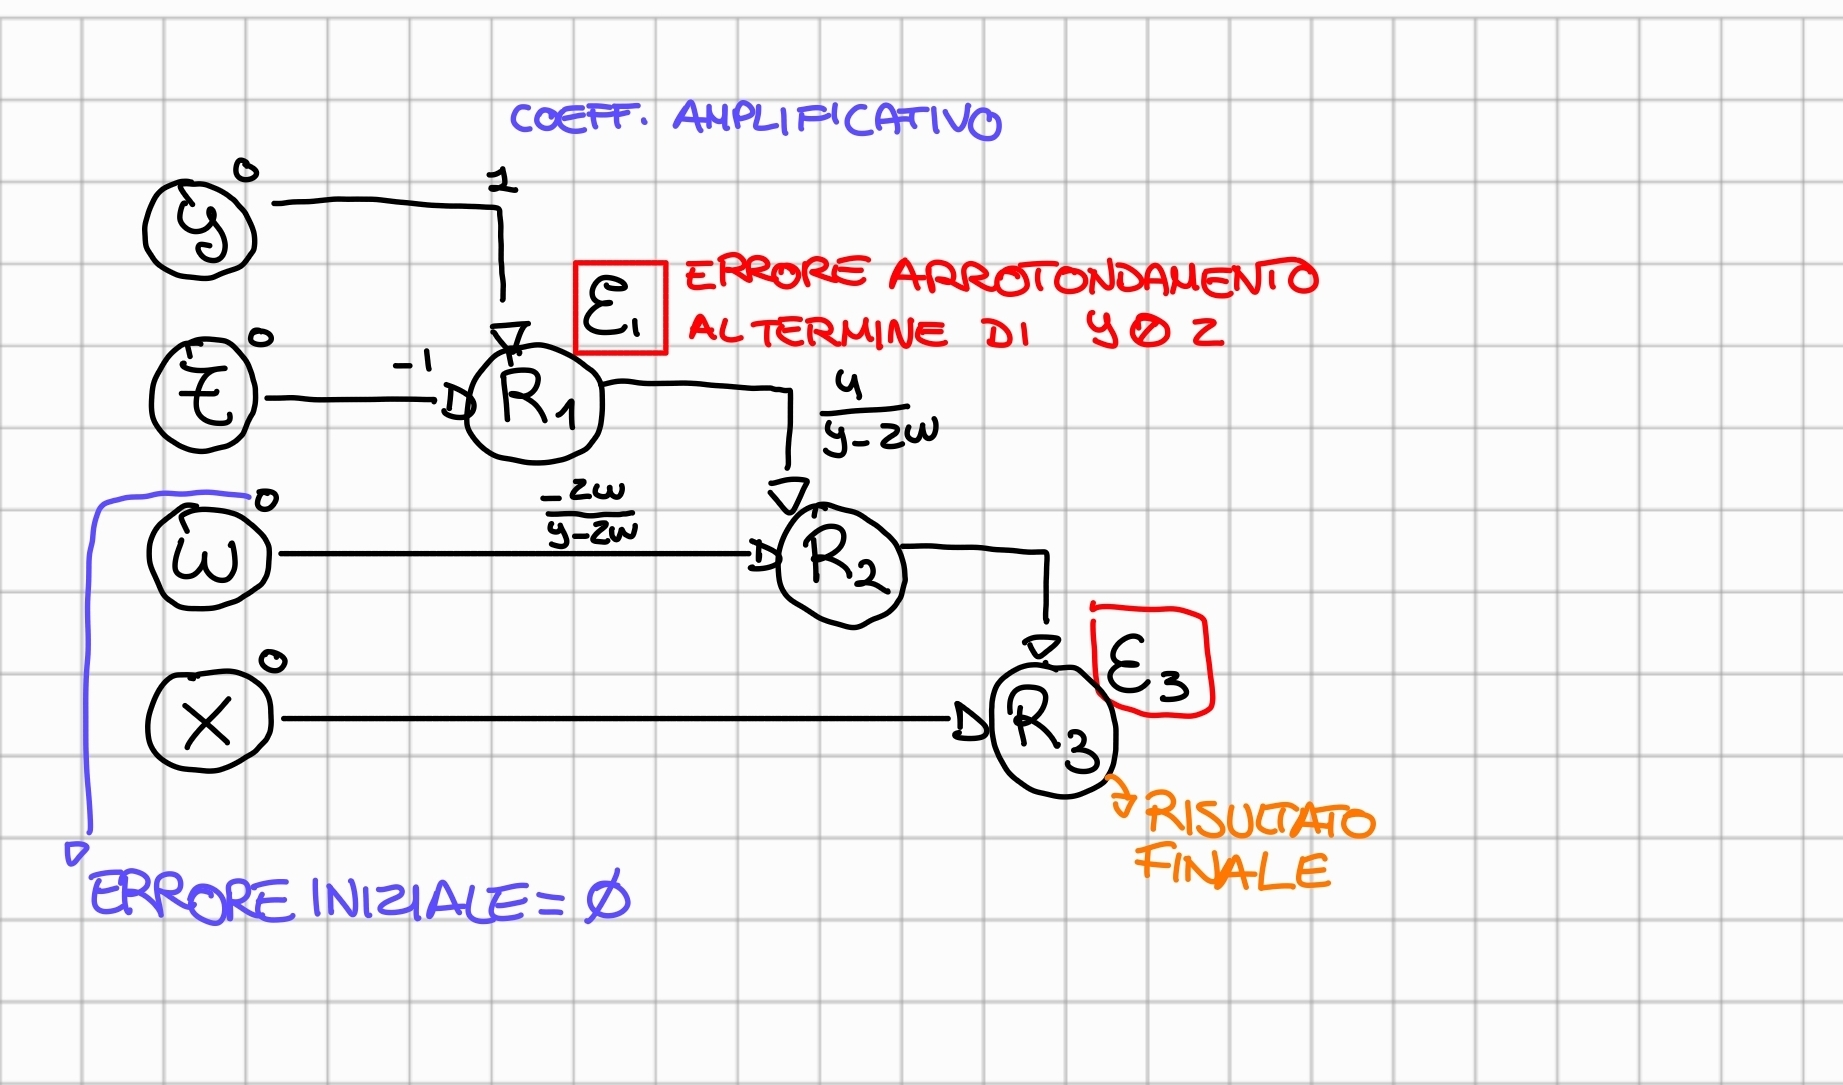
\includegraphics[width=\linewidth]{figura1.jpg}
	\end{figure}
	\paragraph{Spiegazione}
	\begin{itemize}
		\item 
		Sulla sinistra ci sono i valori iniziali $y^0, z^0, w^0, x^0$. In questa analisi ci si concentra solo sull'errore introdotto dall'algoritmo, quindi assumiamo che i dati in ingresso siano esatti.
		\item Il calcolatore esegue la prima operazione: $y \oslash z$.
		\begin{itemize} 
			\item \textbf{Risultato intermedio ($r1$)}: Rappresenta il valore della divisione memorizzato in memoria
			\item \textbf{Errore locale ($\varepsilon_1$)}: Poichè il risultato di $y\div{z}$ potrebbe avere infinite cifre, il computer deve arrotondarlo. Questo arrotondamento genera l'errore locale $\varepsilon_1$
			\item \textbf{Coefficienti sui rami}: Sulle frecce che entrano in $r_1$ i valori $1$ e $-1$ indicano l'errore che si propaga nella divisione.
		\end{itemize}
		\item Il valore ottenuto ($r_1$) viene sottratto a $w: (r_1 \ominus w)$.
		\begin{itemize}
			\item \textbf{Risultato intermedio ($r_2$)}: Adesso è il risultato della parentesi tonda
			\item \textbf{Errore locale ($\varepsilon_2$)} Operazione di sottrazione introduce un nuovo errore di arrotondamento proprio, indicato con $\varepsilon_2$
			\item \textbf{Coefficienti di amplificazione}: Se il denominatore ($y-zw$) è molto piccolo (ovvero se $\frac{y}{z} \approx w$), quesi coefficienti diventano enormi, causando il fenomeno della \textbf{cancellazione numerica} (problema mal condizionato).
		\end{itemize}
		\item Infine, il risultato ($r_2$) viene moltiplicato per $x: x \otimes r_2$.
		\begin{itemize}
			\item \textbf{Risultato finale ($r_3$)}: Valore definitivo restituito dal calcolatore.
			\item \textbf{Errore locale ($\varepsilon_3$)} Anche quest'ultima moltiplicazione introduce un piccolo errore di arrotondamento finale.
			\item \textbf{Propagazione}: La moltiplicazione per sè non amplifica ulteriormente gli errori precedenti in modo drammatico.
		\end{itemize}
	\end{itemize}
	
	
	\[
	\begin{aligned}
		\epsilon_{r_3} &= \epsilon_3 + 1\epsilon_x + 1\epsilon_{r_2} = \epsilon_3 + \epsilon_{r_2} \\
		&= \epsilon_3 + \epsilon_2 + \left( \frac{-zw}{y - zw} \right) \epsilon_w + \frac{y}{y - zw} \epsilon_{r_1} = \\
		&= \epsilon_3 + \epsilon_2 + \frac{y}{y - zw} \epsilon_{r_1} = \epsilon_3 + \epsilon_2 + \frac{y}{y - zw} (\epsilon_1 + 1\epsilon_y - 1\epsilon_z) = \\
		&= \epsilon_3 + \epsilon_2 + \frac{y}{y - zw} \epsilon_1 = \epsilon_a
		\; \; \; \; 
		\text{Sapendo che $\epsilon_w, \epsilon_y, \epsilon_x, \epsilon_z = 0$}
	\end{aligned}
	\]
	
	% Parte superiore: Stima errori assoluti
	\noindent
	Vale che $|\epsilon_1|, |\epsilon_2|, |\epsilon_3| \leq u$. \newline
	Nel caso di errori assoluti: $|\delta_1|, |\delta_2|, |\delta_3| \le u \cdot \max\{|x|, |y|, |z|\}$
	
	\vspace{0.8cm}
	
	% Titolo Esempio
	\noindent
	{\large \textbf{Esempio} $f(x,y) = x^2 - y^2$}
	
	\vspace{0.5cm}
	
	% Struttura a due colonne per gli algoritmi
	\begin{minipage}[t]{0.45\textwidth}
		\textbf{Algoritmo 1:} \\
		$r_1 = x \cdot x$ \\
		$r_2 = y \cdot y$ \\
		$r_3 = r_1 - r_2$
	\end{minipage}
	\hfill
	\begin{minipage}[t]{0.45\textwidth}
		\textbf{Algoritmo 2:} \\
		$r_1 = x + y$ \\
		$r_2 = x - y$ \\
		$r_3 = r_1 \cdot r_2$
	\end{minipage}
	
	\vspace{2cm} 
	
	\begin{figure}[h!]
		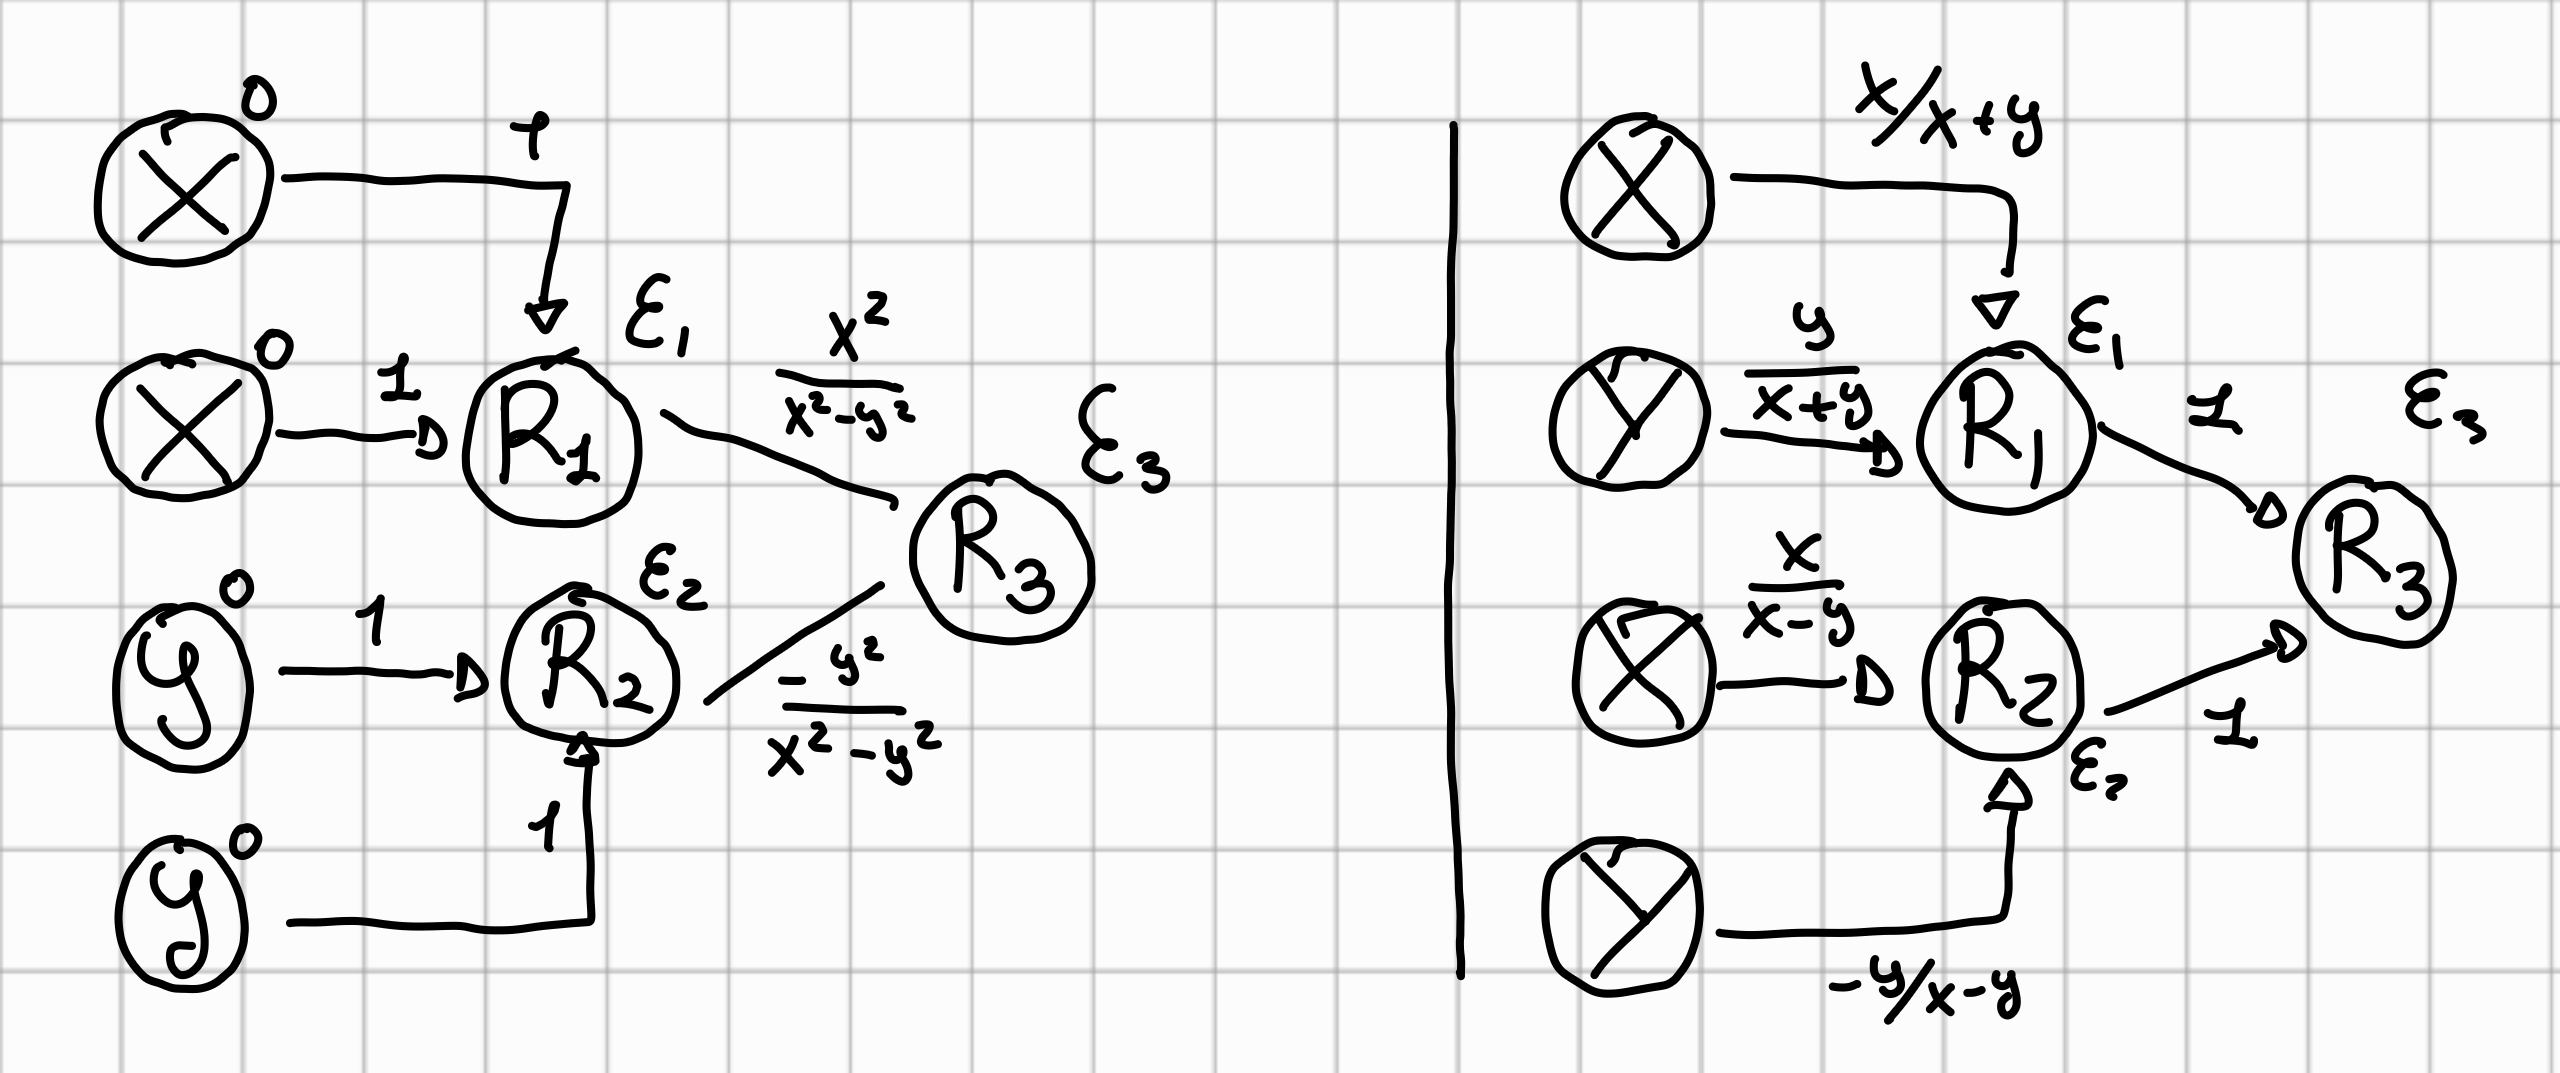
\includegraphics[width=\linewidth]{file2.jpg}
	\end{figure}
	
	\noindent
	\begin{minipage}[t]{0.48\textwidth}
		% Analisi Algoritmo 1
		$$ \epsilon_a = \epsilon_3 + \frac{x^2}{x^2 - y^2} \epsilon_1 - \frac{y^2}{x^2 - y^2} \epsilon_2 $$
	\end{minipage}
	\hfill
	\begin{minipage}[t]{0.48\textwidth}
		% Analisi Algoritmo 2
		$$ \epsilon_a = \epsilon_1 + \epsilon_2 + \epsilon_3 $$
	\end{minipage}
	
	\vspace{1cm}
	
	\noindent
	\textbf{Nota tecnica:} \\
	L'\textbf{Algoritmo 1} è numericamente instabile quando $x \approx y$ a causa del fenomeno della \textit{cancellazione numerica} (i coefficienti dell'errore $\epsilon_1$ ed $\epsilon_2$ tendono all'infinito). \\
	L'\textbf{Algoritmo 2} è invece numericamente stabile poiché l'errore generato $\epsilon_a$ è semplicemente la somma degli errori locali di arrotondamento, indipendentemente dai valori di $x$ e $y$.
	\subsection{Problema Diretto}
	Le tecniche viste per stimare $\epsilon_a$ e $\epsilon_d$ le possiamo usare per stimare
	\begin{align*}
		|\epsilon_f| &\leq |\epsilon_d| + |\epsilon_a| \\
		|\delta_f| &\leq |\delta_d| + |\delta_a|
	\end{align*}
	\begin{tcolorbox}[colback=yellow!10!white, colframe=yellow!50!black]
		\textbf{Problema diretto:} Date $f$, una stima degli errori $\delta_{x_i}$ e un algoritmo, vogliamo stimare $\delta_f$ per $p_0 \in D \subseteq \mathbb{R}^m$
	\end{tcolorbox}
	
	\subsubsection*{Esempio} Consideriamo la funzione $f(x_1, x_2) = \frac{x_1}{x_2}$ definita in un dominio $D$ tale che $x_1 \in [1, 3]$ e $x_2 \in [4, 5]$ ($D = [1,3] \times [4,5], p_0 \in D$). Supponiamo che l'errore sui dati sia limitato da $|\delta_{x_i}| < \frac{1}{2} \cdot 10^{-2}$ per $i = 1, 2$.
	
	\paragraph{Errore inerente:}
	Vogliamo determinare una maggiorazione per l'errore inerente $\delta_d$. Calcoliamo le derivate parziali e i loro estremi superiori nel dominio $D$:
	
	\begin{itemize}
		\item Rispetto a $x_1$: 
		\[ \frac{\partial f}{\partial x_1} = \frac{1}{x_2} \implies A_1 = \sup_{x \in D} \left| \frac{\partial f}{\partial x_1}(x) \right| = \sup_{(x_1,x_2) \in D} \left| \frac{1}{x_2} \right| = \frac{1}{4} \]
		
		\item Rispetto a $x_2$: 
		\[ \frac{\partial f}{\partial x_2} = -\frac{x_1}{x_2^2} \implies A_2 = \sup_{x \in D} \left| \frac{\partial f}{\partial x_2}(x) \right| = \sup_{(x_1,x_2) \in D} \left| -\frac{x_1}{x_2^2} \right| = \frac{3}{16} \]
	\end{itemize}
	
	Dunque, la stima dell'errore totale basata sulla scomposizione $|\delta_f| \leqslant |\delta_a| + |\delta_d|$ diventa:
	\[ 
	|\delta_f| \leqslant |\delta_a| + A_1 |\delta_{x_1}| + A_2 |\delta_{x_2}| = |\delta_a| + \frac{1}{4} \cdot \frac{1}{2} \cdot 10^{-2} + \frac{3}{16} \cdot \frac{1}{2} \cdot 10^{-2} 
	\]
	
	\paragraph{Errore algoritmico:}
	L'errore algoritmico può essere stimato usando la linearizzazione:
	\[ 
	\delta_a = \sum_{j=1}^{m} \frac{\partial f}{\partial x_j}(p_0) \cdot \delta_j \implies |\delta_a| \leqslant \sum_{j=1}^{m} \sup_{p \in D} \left| \frac{\partial f}{\partial x_j}(p) \right| \cdot |\delta_j| 
	\]
	In questo caso specifico (divisione di macchina), l'errore algoritmico è dato dall'arrotondamento del risultato:
	\[ 
	|\delta_a| = \left| \frac{x_1}{x_2} \right| \cdot \frac{1}{2} \cdot 10^{-2} \quad \text{(dato solo dall'errore di troncamento)} 
	\]
	
	\paragraph{Dunque l'errore assoluto:}
	Combinando i risultati ottenuti:
	\[ 
	|\delta_f| \leqslant \left| \frac{x_1}{x_2} \right| \cdot \frac{1}{2} \cdot 10^{-2} + \frac{1}{4} \cdot \frac{1}{2} \cdot 10^{-2} + \frac{3}{16} \cdot \frac{1}{2} \cdot 10^{-2} = \frac{23}{32} \cdot 10^{-2} \leqslant 1
	\]
	
	 \subsection*{Problema Inverso}
	 
	 \begin{tcolorbox}[colback=white, colframe=black]
	 	\textbf{Problema inverso}: dato $\tau > 0$, $f$ e $p_0 \in \mathbb{R}^m$, determinare un algoritmo e un valore di precisione di macchina $u$ tale per cui:
	 	\[ |\delta_f| < \tau \]
	 \end{tcolorbox}
	 
	 \paragraph{Esempio}
	 Sia $f(x_1, x_2) = \frac{x_1}{x_2}$ con dominio $D = [1, 2] \times [-2, -1]$. 
	 Si vuole trovare un algoritmo e una precisione $u$ per cui $|\delta_f| < 10^{-2}$.
	 
	 \medskip
	 \noindent
	 Scegliamo $x_1 \oslash x_2$ come algoritmo e stimiamo gli errori sui dati $|\delta_{x_1}|, |\delta_{x_2}|$:
	 \[ |\delta_{x_i}| \leqslant u \cdot |x_i| \leqslant 2u, \quad i = 1, 2 \]
	 
	 \noindent
	 Calcoliamo i coefficienti di amplificazione (derivate parziali):
	 \begin{itemize}
	 	\item $A_1 = \sup_{D} \left| \frac{\partial f}{\partial x_1} \right| = \sup_{D} \left| \frac{1}{x_2} \right| = 1$
	 	\item $A_2 = \sup_{D} \left| \frac{\partial f}{\partial x_2} \right| = \sup_{D} \left| -\frac{x_1}{x_2^2} \right| = 2$
	 \end{itemize}
	 
	 \paragraph{Stima dell'errore totale:}
	 Utilizzando la scomposizione dell'errore e le maggiorazioni trovate:
	 
	 \[
	 \begin{aligned}
	 	|\delta_f| &\leqslant |\delta_a| + \underbrace{2u}_{|\delta_{x_1}| \cdot A_1} + \underbrace{2u}_{|\delta_{x_2}| \cdot A_2} \\
	 	&\leqslant \max_{D} \left| \frac{x_1}{x_2} \right| \cdot u + 4u = 2u + 4u = 6u
	 \end{aligned}
	 \]
	 
	 \paragraph{Determinazione di $u$:}
	 Per soddisfare la richiesta del problema:
	 \[ |\delta_f| \leqslant 6u \leqslant 10^{-2} \implies u = \frac{1}{6} \cdot 10^{-2} \]
	 
	 \subsection{Funzioni Non Razionali}
	 
	 Se si deve valutare un'espressione matematica \textbf{non razionale} (ad esempio $f(x,y) = e^{\cos(x+y)}$), il calcolatore non può calcolarla esattamente. Si procede quindi scegliendo un'approssimazione razionale $\tilde{f}(x) \approx f(x)$ (ad esempio tramite uno sviluppo di Taylor) e si valuta $\tilde{f}(p_0)$.
	 
	 A causa dell'uso dell'aritmetica floating point e dell'approssimazione della funzione, quello che si ottiene effettivamente è $\tilde{f}_a(p_1)$. Si osserva che l'errore totale può essere scomposto come:
	 
	 \[
	 f(p_0) - \tilde{f}_a(p_1) = \underbrace{f(p_0) - f(p_1)}_{\delta_d} + \underbrace{f(p_1) - \tilde{f}(p_1)}_{\delta_{an}} + \underbrace{\tilde{f}(p_1) - \tilde{f}_a(p_1)}_{\delta_a}
	 \]
	 
	 Dove i contributi sono:
	 \begin{itemize}
	 	\item $\delta_d$: \textbf{Errore inerente} sulla funzione originale $f$;
	 	\item $\delta_{an}$: \textbf{Errore analitico} (dovuto all'approssimazione di $f$ con $\tilde{f}$);
	 	\item $\delta_a$: \textbf{Errore algoritmico} sulla funzione approssimata $\tilde{f}$.
	 \end{itemize}
	 
	 \begin{tcolorbox}[colback=red!5!white]
	 	\[ \delta_f = \delta_d + \delta_a + \delta_{an} \]
	 \end{tcolorbox}
	 
	 \paragraph{Osservazione:} 
	 L'errore inerente è calcolato sulla funzione originale ($f$), mentre l'errore algoritmico è calcolato sulla funzione approssimata $\tilde{f}$ (di conseguenza, per stimare $\delta_a$ serve un'analisi del grafo computazionale dell'algoritmo che valuta effettivamente $\tilde{f}$).
	 
	 Con tecniche simili a quanto visto nel caso razionale, si dimostra che (a meno di termini trascurabili di ordine superiore) per l'\textbf{errore relativo} vale:
	 
	 \begin{equation}
	 	\epsilon_f := \frac{f(p_0) - \tilde{f}_a(p_1)}{f(p_0)} \qquad \epsilon_f \approx \epsilon_d + \epsilon_a + \epsilon_{an}
	 \end{equation}
	 
	 dove l'errore relativo analitico è definito come:
	 \begin{equation}
	 	\epsilon_{an} := \frac{f(p_1) - \tilde{f}(p_1)}{f(p_1)}
	 \end{equation}
	 
	 \paragraph{Stima dell'errore analitico}
	 Le quantità $\delta_{an}$ ed $\epsilon_{an}$ si stimano utilizzando i risultati della \textbf{teoria dell'approssimazione}. L'esempio più comune (e l'unico che verrà trattato nel corso) è l'approssimazione di una funzione mediante il \textbf{polinomio di Taylor}, per funzioni del tipo $f: \mathbb{R} \to \mathbb{R}$.
	
	\paragraph{Reminder:} 
	Data una funzione $f: \mathbb{R} \to \mathbb{R}$, con $f \in C^{n+1}(\mathbb{R})$ e un punto di centro $x_0 \in \mathbb{R}$, allora:
	
	\begin{equation}
		f(x) = \underbrace{\sum_{j=0}^{n} \frac{f^{(j)}(x_0)}{j!} \cdot (x-x_0)^j}_{\text{Polinomio di grado } n} + \underbrace{\frac{f^{(n+1)}(\eta)}{(n+1)!} (x-x_0)^{n+1}}_{\text{Resto di Lagrange}}
	\end{equation}
	
	Dove:
	\begin{itemize}
		\item La parte polinomiale sarà la nostra \textbf{funzione razionale} $\tilde{f}(x)$ che usiamo per approssimare $f(x)$.
		\item Il \textbf{Resto di Lagrange} è il termine che serve per stimare l'errore analitico.
		\item $\eta$ è un valore incognito compreso nell'intervallo tra $x$ e $x_0$ (ovvero $\eta \in [x, x_0]$ oppure $\eta \in [x_0, x]$).
	\end{itemize}
	
	\paragraph{Osservazione:}
	In questo contesto, l'errore analitico assoluto e relativo si identificano direttamente con il resto della serie di Taylor:
	
	\begin{tcolorbox}[colback=blue!5!white, colframe=blue!75!black]
		\begin{align}
			\delta_{an}(x) &= \frac{f^{(n+1)}(\eta)}{(n+1)!} (x-x_0)^{n+1} \\
			\epsilon_{an}(x) &= \frac{f^{(n+1)}(\eta)}{(n+1)!} \frac{(x-x_0)^{n+1}}{f(x)}
		\end{align}
	\end{tcolorbox}
	\paragraph{Esempio: Approssimazione della Funzione Esponenziale}
	
	Consideriamo l'approssimazione della funzione $f(x) = e^x$ mediante il suo polinomio di Taylor di grado $n=2$ centrato in $x_0=0$:
	\[ \tilde{f}(x) = 1 + x + \frac{x^2}{2} \]
	
	Vogliamo stimare quanto sia grande l'errore relativo analitico $|\epsilon_{an}|$ e trovare una sua maggiorazione per $x \in [-1, 1]$.
	
	\paragraph{Calcolo dell'errore analitico assoluto:}
	Utilizzando il resto di Lagrange con $n=2$ (dove la derivata terza di $e^x$ è ancora $e^x$):
	\[ \delta_{an}(x) = e^x - \left( 1 + x + \frac{x^2}{2} \right) = \frac{f^{(3)}(\eta)}{3!} x^3 = \frac{e^\eta x^3}{6} \]
	con $\eta$ compreso tra $0$ e $x$.
	
	\paragraph{Calcolo dell'errore analitico relativo:}
	Dividendo per il valore esatto della funzione $f(x) = e^x$:
	\[ \epsilon_{an}(x) = \frac{\delta_{an}(x)}{f(x)} = \frac{e^\eta x^3}{6 e^x} \]
	
	\paragraph{Maggiorazione dell'errore nell'intervallo $[-1, 1]$:}
	Per trovare un limite superiore, cerchiamo i valori massimi dei componenti per $x, \eta \in [-1, 1]$:
	\[ 
	\max_{x \in [-1, 1]} |\epsilon_{an}(x)| \leqslant \max_{\eta \in [-1, 1]} e^\eta \cdot \max_{x \in [-1, 1]} \left| \frac{x^3}{6 e^x} \right| \leqslant \frac{e}{6} \cdot \frac{\max_{x \in [-1, 1]} |x^3|}{\min_{x \in [-1, 1]} e^x} 
	\]
	
	Sostituendo i valori estremi nel dominio:
	\[ 
	|\epsilon_{an}(x)| \leqslant \frac{e}{6} \cdot \frac{1}{e^{-1}} = \frac{e^2}{6} \approx 1.23 
	\]
	
	\begin{tcolorbox}[colback=orange!5!white, colframe=orange!75!black]
		\textbf{Conclusione:} L'errore ottenuto ($\approx 123\%$) non è molto accurato. Questo indica che un polinomio di secondo grado non è sufficiente per approssimare bene l'esponenziale su un intervallo ampio come $[-1, 1]$.
	\end{tcolorbox}
	
	\paragraph{Generalizzazione al Grado $n$}
	
	Se considerassimo il polinomio di Taylor di grado $n$, otterremmo un errore assoluto analitico espresso come:
	\begin{equation}
		\delta_{an}(x) = \frac{e^{\eta} x^{n+1}}{(n+1)!}
	\end{equation}
	
	Ragionando come nel caso precedente per la maggiorazione dell'errore relativo nell'intervallo $x \in [-1, 1]$, si ottiene:
	\begin{equation}
		|\epsilon_{an}(x)| \leqslant \frac{e^2}{(n+1)!} \xrightarrow[n \to +\infty]{} 0
	\end{equation}
	
	Questo limite ci conferma che all'aumentare del grado del polinomio, l'approssimazione diventa sempre più precisa, tendendo a zero.
	
	\paragraph{Esempio con $n=4$}
	Considerando il polinomio di quarto grado:
	\[ \tilde{f}(x) = 1 + x + \frac{x^2}{2} + \frac{x^3}{6} + \frac{x^4}{24} \]
	
	Per $x \in [-1, 1]$, si ottiene una stima dell'errore molto più contenuta:
	\begin{equation}
		|\epsilon_{an}(x)| \leqslant \frac{e^2}{5!} = \frac{e^2}{120} \approx 0,061
	\end{equation}
	
	\begin{tcolorbox}[colback=green!5!white, colframe=green!50!black]
		\textbf{Conclusione finale}: Passando dal grado $n=2$ al grado $n=4$, l'errore relativo è sceso da circa $1,23$ ($123\%$) a $0,061$ ($6,1\%$). Questo rende l'approssimazione decisamente più accettabile per fini computazionali.
	\end{tcolorbox}
	
	\section{Richiami di Algebra Lineare}
	L'oggetto di interesse è spesso un vettore $x \in \mathbb{R}^n$, oppure si considerano funzioni $f:\mathbb{R}^n \rightarrow \mathbb{R}^m$. 
	
	Una funzione $f:\mathbb{R}^n \rightarrow \mathbb{R}^m$ si dice lineare se soddisfa le seguenti proprietà:
	\begin{align*}
		f(x+y) &= f(x) + f(y) \quad \forall x, y \in \mathbb{R}^n \\
		f(\lambda x) &= \lambda f(x) \quad \forall \lambda \in \mathbb{R}, \; \forall x \in \mathbb{R}^n
	\end{align*}
	allora $\exists{!} A \in \mathbb{R}^{m \times n}$ tale per cui $\forall x \in \mathbb{R}^n$ vale $f(x) = A \cdot x$
	\[
	A = \begin{bmatrix}
		a_{11} & a_{12} & a_{13} & \dots  & a_{1n} \\
		a_{21} & a_{22} & a_{23} & \dots  & a_{2n} \\
		\vdots & \vdots & \vdots & \ddots & \vdots \\
		a_{n1} & a_{n2} & a_{n3} & \dots  & a_{nn}
	\end{bmatrix}
	\]
	\begin{itemize}
		\item Se $m = n \rightarrow $ La matrice è \textbf{Quadrata}
		\item Se $m \neq n \rightarrow$ La matrice è \textbf{Rettangolare}
	\end{itemize}
	
	\begin{tcolorbox}[title=Definizione]
		$x_1,...,x_s \in \mathbb{C}^n$ si dicono linearmente indipendenti se:
		\begin{align*}
			\sum_{i=1}^{s} \alpha_i \cdot x_i = 0 \iff \alpha_1 = \alpha_2 = \dots = \alpha_s = 0
		\end{align*}
	\end{tcolorbox}
	Viceversa $x_1, \dots, x_s$ si dicono linearmente dipendenti se $\exists j \in \{1, \dots, s\}$ tale per cui:
	\[
	x_j = \sum_{i \neq j} \alpha_i x_i \quad \text{per qualche } \alpha_i \in \mathbb{C}
	\]
	
	\begin{tcolorbox}[title=Definizione]
		Un insieme di $n$ vettori linearmente indipendenti in $\mathbb{C}^n$ si dice \textbf{base}.
	\end{tcolorbox}
	
	\begin{tcolorbox}[title=Definizione]
		Dati $x, y \in \mathbb{C}^n$, si definisce \textbf{prodotto scalare} la quantità:
		\[
		\langle x, y \rangle = \sum_{i=1}^{n} x_i \overline{y}_i
		\]
		Di conseguenza, si ha:
		\[
		\langle x, x \rangle = \|x\|_2^2 = \sum_{i=1}^{n} |x_i|^2
		\]
	\end{tcolorbox} 
	\begin{tcolorbox}[title=Definizione]
		Due vettori $x, y$ si dicono \textbf{ortogonali} se vale:
		\[
		\langle x, y \rangle = 0
		\]
	\end{tcolorbox}
	
	\textbf{Osservazione:} Se contiamo le operazioni di un prodotto scalare, queste sono $n$ prodotti e $n-1$ somme e scriviamo che il suo costo è $\mathcal{O}(n)$ oppure $\mathcal{O}(2n)$. Significa che:
	\[
	\lim_{n \to +\infty} \frac{\text{costo prodotto scalare}}{n} = \text{costante finita} \neq 0
	\]
	\begin{tcolorbox}[title=Definizione (Trasposta e Trasposta Coniugata)]
		Sia $A \in \mathbb{C}^{n \times m}$. Si definiscono:
		\begin{itemize}
			\item \textbf{Trasposta}: $A^T \in \mathbb{C}^{m \times n}$ tale che:
			\[
			(A^T)_{ij} = A_{ji}
			\]
			\item \textbf{Hermitiana} (trasposta coniugata): $A^H \in \mathbb{C}^{m \times n}$ tale che:
			\[
			(A^H)_{ij} = \overline{A_{ji}}
			\]
		\end{itemize}
	\end{tcolorbox}
	
	\subsubsection*{Esempi}
	
	1. Matrice reale:
	\[
	A = \begin{bmatrix} 1 & 7 & 8 \\ 4 & 2 & 9 \\ 5 & 6 & 3 \end{bmatrix} \implies A^T = \begin{bmatrix} 1 & 4 & 5 \\ 7 & 2 & 6 \\ 8 & 3 & 3 \end{bmatrix}
	\]
	
	2. Matrice complessa:
	\[
	A = \begin{bmatrix} 1 & 2 & 3i \\ -i & 1+i & 0 \\ 4 & 0 & 3 \end{bmatrix} \implies A^H = \begin{bmatrix} 1 & i & 4 \\ 2 & 1-i & 0 \\ -3i & 0 & 3 \end{bmatrix}
	\]
	
	\paragraph{In MATLAB:}
	\begin{itemize}
		\item \texttt{A'} $\rightsquigarrow A^H$ (operatore trasposta coniugata)
		\item \texttt{A.'} $\rightsquigarrow A^T$ (operatore trasposta semplice)
	\end{itemize}
	
	Per definire una matrice elemento per elemento in MATLAB:
	\begin{verbatim}
		A = [ 1 2 3 ; 4 5 6 ];
	\end{verbatim}
	Che corrisponde a:
	\[
	A = \begin{bmatrix} 1 & 2 & 3 \\ 4 & 5 & 6 \end{bmatrix}
	\]
	\begin{tcolorbox}[title=Definizione (Matrice Diagonale)]
		Una matrice si dice \textbf{diagonale} se ha elementi nulli fuori dalla diagonale principale, ovvero:
		\[
		a_{ij} = 0 \quad \forall i \neq j
		\]
	\end{tcolorbox}
	
	\paragraph{In MATLAB:} Il comando \texttt{diag(v)} crea una matrice con elementi uguali a $0$ tranne che sulla diagonale principale, dove inserisce gli elementi del vettore \texttt{v}.
	
	\begin{tcolorbox}[title=Definizione (Matrice Triangolare)]
		Una matrice quadrata si dice \textbf{triangolare superiore} (risp. \textbf{inferiore}) se ha tutti gli elementi nulli sotto (risp. sopra) la diagonale principale:
		\begin{itemize}
			\item \textbf{Triangolare Superiore ($U$):}
			\[
			U = \begin{bmatrix} 
				u_{11} & \dots & u_{1n} \\ 
				& \ddots & \vdots \\ 
				0 & & u_{nn} 
			\end{bmatrix}
			\]
			\item \textbf{Triangolare Inferiore ($L$):}
			\[
			L = \begin{bmatrix} 
				l_{11} & & 0 \\ 
				\vdots & \ddots & \\ 
				l_{n1} & \dots & l_{nn} 
			\end{bmatrix}
			\]
		\end{itemize}
	\end{tcolorbox}
	
	\paragraph{In MATLAB:} Esistono i comandi \texttt{triu} (\textit{triangle upper}) e \texttt{tril} (\textit{triangle lower}) che estraggono rispettivamente la parte triangolare superiore o inferiore di una matrice data in input.
	\section*{Costo Computazionale e Proprietà del Prodotto}
	
	\textbf{Osservazione:} Dato che la matrice prodotto $C = A \cdot B$ ha $m \times p$ entrate, e ogni entrata richiede un prodotto scalare tra una riga di $A$ (lunga $n$) e una colonna di $B$, il costo del prodotto è:
	\[
	A \cdot B \implies \mathcal{O}(m \cdot n \cdot p)
	\]
	Se consideriamo matrici quadrate di ordine $n$ ($m=n=p$), il costo diventa $\mathcal{O}(n^3)$.
	
	\textbf{Osservazione (Matrici Sparse o a Blocchi):} Può essere utile decomporre le matrici se una delle due ha molti zeri o se è strutturata a blocchi:
	\[
	A = \begin{bmatrix} A_1 \\ \hline A_2 \end{bmatrix} \implies AB = \begin{bmatrix} A_1 B \\ \hline A_2 B \end{bmatrix}, \quad B = [B_1 | \dots | B_n] \implies AB = [AB_1 | \dots | AB_n]
	\]
	
	\subsubsection*{Proprietà del Prodotto}
	\begin{itemize}
		\item \textbf{Non commutatività:} In generale $AB \neq BA$.
		\item \textbf{Associatività:} $(A \cdot B) \cdot C = A \cdot (B \cdot C)$.
		\item \textbf{Distributività:} $(A + B) \cdot C = AC + BC$.
	\end{itemize}
	
	---
	
	\section*{Analisi del Costo Computazionale}
	
	\textbf{Osservazione:} Anche se la moltiplicazione è associativa, l'ordine con cui si eseguono le operazioni può influenzare drasticamente il costo.
	Siano $A \in \mathbb{C}^{m \times n}, B \in \mathbb{C}^{n \times p}, C \in \mathbb{C}^{p \times q}$.
	\begin{enumerate}
		\item $(A \cdot B) \cdot C \implies \mathcal{O}(mnp + mpq)$
		\item $A \cdot (B \cdot C) \implies \mathcal{O}(npq + mnq)$
	\end{enumerate}
	
	Se, ad esempio, $m=1$ (vettore riga) e $n=p=q$ sono grandi, il primo metodo costa $\mathcal{O}(n^2)$ mentre il secondo $\mathcal{O}(n^3)$
	
	---
	
	\begin{tcolorbox}[title=Definizione: Determinante]
		Data una matrice quadrata $A \in \mathbb{C}^{n \times n}$, il determinante si definisce ricorsivamente (Sviluppo di Laplace):
		\[
		\det(A) = \begin{cases} a_{11} & n=1 \\ \sum_{j=1}^{n} (-1)^{i+j} a_{ij} \det(A_{ij}) & n > 1 \end{cases}
		\]
		dove $A_{ij}$ è la sottomatrice ottenuta cancellando la riga $i$ e la colonna $j$
	\end{tcolorbox}
	
	\paragraph{In MATLAB:} Si usa la funzione \texttt{det(A)}
	
	\subsubsection*{Casi Particolari e Proprietà}
	\begin{itemize}
		\item Per matrici \textbf{triangolari} o \textbf{diagonali}: $\det(A) = \prod_{i=1}^n a_{ii}$. In questo caso il costo è solo $\mathcal{O}(n)$
		\item $\det(A) = \det(A^T)$
		\item $\det(A^H) = \overline{\det(A)}$
		\item $\det(\lambda A) = \lambda^n \det(A)$
	\end{itemize}
	
	Una matrice $A$ si dice \textbf{singolare} se $\det(A) = 0$
	
	---
	
	\begin{tcolorbox}[title=Definizione: Rango]
		Il \textbf{rango} di una matrice $A \in \mathbb{C}^{m \times n}$ è definito equivalentemente come:
		\begin{itemize}
			\item Numero di colonne (o righe) linearmente indipendenti.
			\item Dimensione massima di un minore non nullo (sottomatrice quadrata con $\det \neq 0$)
			\item Dimensione dell'immagine $Im(A) = \{y \in \mathbb{C}^m : \exists x, y = Ax\}$
		\end{itemize}
	\end{tcolorbox}
	
	\textbf{Teorema di Binet-Cauchy:} $\det(A \cdot B) = \det(A) \cdot \det(B)$
	
	---
	
	\begin{tcolorbox}[title=Definizione: Matrice Inversa]
		Sia $A \in \mathbb{C}^{n \times n}$ non singolare. Si definisce l'inversa $A^{-1}$ la matrice tale che:
		\[
		A \cdot A^{-1} = A^{-1} \cdot A = I
		\]
		dove $I = \text{diag}(1, \dots, 1)$ è la matrice identità
	\end{tcolorbox}
	
	\paragraph{Proprietà dell'inversa:}
	\begin{enumerate}
		\item $A^{-1}$ esiste $\iff \det(A) \neq 0 \iff$ rango$(A) = n$
		\item $\det(A^{-1}) = \frac{1}{\det(A)}$
		\item $(AB)^{-1} = B^{-1}A^{-1}$
	\end{enumerate}
	
	\paragraph{In MATLAB:} \texttt{inv(A)} per l'inversa e \texttt{eye(n)} per la matrice identità.
	\section*{Proprietà dell'Inversa e Classi di Matrici}
	
	\textbf{Proprietà dell'Inversa:}
	\begin{enumerate}
		\item $A^{-1}$ esiste $\iff \det(A) \neq 0 \iff$ le righe/colonne di $A$ sono linearmente indipendenti $\iff \text{rank}(A) = n$
		\item Per il teorema di Binet-Cauchy, $\det(A \cdot A^{-1}) = \det(I) = 1$, da cui $\det(A^{-1}) = \frac{1}{\det(A)}$
		\item $(A \cdot B)^{-1} = B^{-1} \cdot A^{-1}$ (e analogamente per la trasposta $(AB)^T = B^T A^T$ e l'hermitiana $(AB)^H = B^H A^H$)
	\end{enumerate}
	
	\begin{tcolorbox}[title=Definizione: Matrici Speciali ($\mathbb{C}^{n \times n}$)]
		Una matrice $A \in \mathbb{C}^{n \times n}$ si dice:
		\begin{itemize}
			\item \textbf{Hermitiana} se $A = A^H$
			\item \textbf{Unitaria} se $AA^H = A^H A = I$ (ovvero $A^H = A^{-1}$)
			\item \textbf{Normale} se $AA^H = A^H A$
		\end{itemize}
		\textit{Nota:} Le matrici hermitiane e unitarie sono sottoclassi delle matrici normali
	\end{tcolorbox}
	
	\begin{tcolorbox}[title=Definizione: Caso Reale ($\mathbb{R}^{n \times n}$)]
		Se $A \in \mathbb{R}^{n \times n}$, le definizioni precedenti diventano:
		\begin{itemize}
			\item \textbf{Simmetrica} se $A = A^T$
			\item \textbf{Ortogonale} se $A^T A = AA^T = I$
		\end{itemize}
	\end{tcolorbox}
	
	---
	
	\section*{Matrici di Permutazione}
	
	\begin{tcolorbox}[title=Definizione]
		Una matrice $P \in \mathbb{R}^{n \times n}$ si dice \textbf{di permutazione} se è ottenuta dalla matrice identità permutando l'ordine delle righe o delle colonne
	\end{tcolorbox}
	
	\textbf{Proprietà:}
	\begin{itemize}
		\item Ogni matrice di permutazione è ortogonale: $P^T P = P P^T = I$
		\item \textbf{Effetto del prodotto:} Moltiplicare $PA$ scambia le \textbf{righe} di $A$, mentre $AP$ scambia le \textbf{colonne} di $A$
	\end{itemize}
	
	\textit{Esempio:} Se $P = \begin{bmatrix} 0 & 1 & 0 \\ 0 & 0 & 1 \\ 1 & 0 & 0 \end{bmatrix}$ e $A = \begin{bmatrix} 1 & 4 & 7 \\ 2 & 5 & 8 \\ 3 & 6 & 9 \end{bmatrix}$, allora $PA = \begin{bmatrix} 2 & 5 & 8 \\ 3 & 6 & 9 \\ 1 & 4 & 7 \end{bmatrix}$
	
	---
	
	\section*{Sistemi Lineari}
	
	Un sistema di $m$ equazioni in $n$ incognite si scrive come $Ax = b$, dove $A \in \mathbb{C}^{m \times n}$, $x \in \mathbb{C}^n$ è il vettore delle incognite e $b \in \mathbb{C}^m$ è il termine noto.
	
	\begin{tcolorbox}[title=Teorema di Rouché-Capelli]
		Il sistema $Ax = b$ ammette soluzione se e solo se:
		\[ \text{rank}(A) = \text{rank}(A|b) \]
		dove $[A|b]$ è la matrice aumentata ottenuta aggiungendo $b$ come ultima colonna ad $A$
	\end{tcolorbox}
	
	\textbf{Unicità della soluzione:}
	\begin{itemize}
		\item Se $\text{rank}(A) = n$ (numero incognite), la soluzione è \textbf{unica}
		\item Se $\text{rank}(A) < n$, esistono \textbf{infinite soluzioni} che formano uno spazio affine di dimensione $n - \text{rank}(A)$
	\end{itemize}
	
	\textbf{Casi particolari:}
	\begin{itemize}
		\item \textbf{Sistema Omogeneo ($b=0$):} ammette sempre almeno la soluzione nulla $x=0$.
		\item \textbf{Sistema Sovradeterminato:} $m > n$.
		\item \textbf{Sistema Sottodeterminato:} $m < n$.
	\end{itemize}
	
	---
	
	\section*{Esercizio MATLAB: Sviluppo di Laplace}
	
	\textbf{Consegna:} Scrivere una funzione \texttt{my\_det(A)} che calcoli il determinante facendo lo sviluppo di Laplace sulla prima riga:
	\[ \det(A) = \sum_{j=1}^{n} (-1)^{1+j} a_{1j} \det(A_{1j}) \]
	
	\textbf{Suggerimenti (Hint):}
	\begin{itemize}
		\item Definire la funzione in modo \textbf{ricorsivo}
		\item Caso base: se $n=1$, $\det(A) = a_{11}$
		\item Per ottenere la sottomatrice $A_{1j}$ in MATLAB, escludere la prima riga e la colonna $j$ usando gli indici: \texttt{A(2:n, [1:j-1, j+1:n])}
	\end{itemize}
	...
	
	\section{Autovalori e Autovettori}
	
	\begin{tcolorbox}[title=Definizione]
		Siano $A \in \mathbb{C}^{n \times n}$ e $\lambda \in \mathbb{C}$. Si dice che $\lambda$ è un \textbf{autovalore} di $A$ se esiste un vettore non nullo $v \in \mathbb{C}^n, v \neq 0$ tale che:
		\begin{equation}
			A v = \lambda v
		\end{equation}
		Il vettore $v$ associato a $\lambda$ si dice \textbf{autovettore}. La coppia $(\lambda, v)$ è detta \textbf{autocoppia}.
	\end{tcolorbox}
	
	\paragraph{Esistenza degli autovalori:} 
	Dalla relazione $Av = \lambda v$ segue che $(A - \lambda I)v = 0$. Poiché per definizione $v \neq 0$, il sistema lineare omogeneo associato deve ammettere soluzioni non banali. Per il teorema di Cramer, ciò accade se e solo se la matrice $(A - \lambda I)$ è singolare:
	\begin{equation*}
		p_A(\lambda) = \det(A - \lambda I) = 0 \quad \leadsto \quad \textbf{Equazione Caratteristica}
	\end{equation*}
	
	\paragraph{Esempio:} 
	Sia $A = \begin{bmatrix} 1 & 3 \\ 0 & 4 \end{bmatrix}$. Calcoliamo il polinomio caratteristico:
	\[
	A - \lambda I = \begin{bmatrix} 1-\lambda & 3 \\ 0 & 4-\lambda \end{bmatrix} \implies \det(A - \lambda I) = (1-\lambda)(4-\lambda) = \lambda^2 - 5\lambda + 4
	\]
	Le radici $\lambda_1 = 1$ e $\lambda_2 = 4$ sono gli autovalori di $A$.
	
	\medskip
	\noindent In generale, $p_A(\lambda)$ è un \textbf{polinomio di grado $n$} in $\lambda$. Per il Teorema Fondamentale dell'Algebra, esso ha esattamente $n$ radici complesse (contate con la loro molteplicità). Di conseguenza, ogni matrice quadrata di ordine $n$ possiede esattamente $n$ autovalori.
	
	\begin{tcolorbox}[title=Definizione: Molteplicità Algebrica]
		Si definisce \textbf{molteplicità algebrica} $\alpha(\lambda_i)$ di un autovalore $\lambda_i$ la sua molteplicità come radice del polinomio caratteristico $p_A(\lambda)$.
	\end{tcolorbox}
	
	\paragraph{Proprietà degli Autovalori:} 
	Se $\lambda_1, \dots, \lambda_n$ sono gli autovalori di $A$ (ripetuti secondo la loro molteplicità), valgono le seguenti relazioni fondamentali:
	\begin{itemize}
		\item \textbf{Traccia:} $\gamma_1 = \text{tr}(A) = \sum_{j=1}^n a_{jj} = \sum_{j=1}^n \lambda_j$
		\item \textbf{Determinante:} $\gamma_n = \det(A) = \prod_{j=1}^n \lambda_j$
	\end{itemize}
	\textit{Osservazione:} Una matrice è singolare ($\det(A)=0$) se e solo se ammette almeno un autovalore nullo.
	
	\subsection{Autospazi e Molteplicità Geometrica}
	Se $v$ è un autovettore associato a $\lambda$, allora anche ogni suo multiplo $\theta v$ (con $\theta \in \mathbb{C} \setminus \{0\}$) soddisfa l'equazione $A(\theta v) = \lambda(\theta v)$. L'insieme di tutti gli autovettori associati a $\lambda$, unitamente al vettore nullo, costituisce un sottospazio vettoriale di $\mathbb{C}^n$.
	
	\begin{tcolorbox}[title=Definizione: Molteplicità Geometrica, colback=white]
		Si definisce \textbf{autospazio} relativo a $\lambda$ il sottospazio:
		\[ V_\lambda = \ker(A - \lambda I) \]
		La sua dimensione è detta \textbf{molteplicità geometrica} $\gamma(\lambda)$:
		\begin{equation}
			\gamma(\lambda) := \dim(\ker(A - \lambda I)) = n - \text{rank}(A - \lambda I)
		\end{equation}
	\end{tcolorbox}
	
	\paragraph{Proprietà delle molteplicità:}
	Per ogni autovalore $\lambda$ di una matrice $A$, sussiste sempre la seguente catena di disuguaglianze:
	\begin{equation}
		1 \le \gamma(\lambda) \le \alpha(\lambda) \le n
	\end{equation}
	Se per un autovalore si ha $\gamma(\lambda) < \alpha(\lambda)$, la matrice si dice \textbf{difettiva}. Se invece $\gamma(\lambda) = \alpha(\lambda)$ per tutti gli autovalori, la matrice è \textbf{diagonalizzabile}.
	\section{Similitudine tra Matrici}
	
	\begin{tcolorbox}[title=Definizione: Matrici Simili]
		Due matrici $A, B \in \mathbb{C}^{n \times n}$ si dicono \textbf{simili} (e si indica con $A \sim B$) se esiste una matrice non singolare $S \in \mathbb{C}^{n \times n}$ ($\det(S) \neq 0$) tale che:
		\begin{equation}
			B = S^{-1} A S
		\end{equation}
	\end{tcolorbox}
	
	\paragraph{Teorema:} 
	Se $A \sim B$, allora $A$ e $B$ hanno lo \textbf{stesso polinomio caratteristico} (e quindi gli stessi autovalori con le stesse molteplicità algebriche). 
	Inoltre, se $v$ è un autovettore di $A$ associato all'autovalore $\lambda$, allora $w = S^{-1}v$ è un autovettore di $B$ associato allo stesso $\lambda$.
	
	\paragraph{Dimostrazione (Invarianza del Polinomio Caratteristico):}
	Sfruttando le proprietà del determinante e l'identità $I = S^{-1} S$:
	\begin{align*}
		\det(B - \lambda I) &= \det(S^{-1} A S - \lambda I) \\
		&= \det(S^{-1} A S - \lambda S^{-1} S) \\
		&= \det(S^{-1} (A - \lambda I) S) \\
		\intertext{Per il teorema di Binet:}
		&= \det(S^{-1}) \cdot \det(A - \lambda I) \cdot \det(S) \\
		&= \frac{1}{\det(S)} \cdot \det(S) \cdot \det(A - \lambda I) \\
		&= \det(A - \lambda I)
	\end{align*}
	Poiché i polinomi caratteristici coincidono, le radici (autovalori) sono le stesse.
	
	\paragraph{Trasformazione degli autovettori:}
	Sia $(\lambda, v)$ un'autocoppia per $A$, ovvero $Av = \lambda v$. Verifichiamo che $w = S^{-1}v$ sia autovettore per $B$:
	\[
	B w = (S^{-1} A S) (S^{-1} v) = S^{-1} A (S S^{-1}) v = S^{-1} A v = S^{-1} (\lambda v) = \lambda (S^{-1} v) = \lambda w
	\]
	Questo dimostra che $w$ soddisfa la definizione di autovettore per $B$ con lo stesso autovalore $\lambda$.
	
	\begin{tcolorbox}[title=Osservazione: Diagonalizzabilità, colback=blue!5!white]
		Una matrice $A$ si dice \textbf{diagonalizzabile} se è simile a una matrice diagonale $D$. In tal caso:
		\[ D = S^{-1} A S \implies A = S D S^{-1} \]
		dove $D$ contiene gli autovalori sulla diagonale e $S$ ha come colonne gli autovettori linearmente indipendenti di $A$.
	\end{tcolorbox}
	\paragraph{Dimostrazione (Trasformazione degli autovettori):}
	Sia $(\lambda, v)$ un'autocoppia per $A$. Verifichiamo che $S^{-1}v$ sia autovettore per $B = S^{-1}AS$:
	\begin{equation*}
		B (S^{-1} v) = S^{-1} A \underbrace{(S \cdot S^{-1})}_{I} v = S^{-1} \underbrace{(A v)}_{\lambda v} = S^{-1} \lambda v = \lambda (S^{-1} v)
	\end{equation*}
	Da cui segue che $S^{-1}v$ è autovettore per $B$ associato all'autovalore $\lambda$. $\square$
	
	\vspace{0.5cm}
	
	\begin{tcolorbox}[title=Esempio: Matrice Diagonale, colback=white]
		Sia $A$ una matrice diagonale di ordine $n$:
		\[
		A = \begin{bmatrix}
			\lambda_1 & & 0 \\
			& \ddots & \\
			0 & & \lambda_n
		\end{bmatrix}
		\]
		Per una matrice in questa forma, gli autovalori sono esattamente gli elementi $\lambda_i$ sulla diagonale. Gli autovettori associati sono i vettori della \textbf{base canonica} $e_i$.
		
		\medskip
		Prendendo ad esempio il primo vettore della base canonica $e_1$:
		\[
		A \begin{bmatrix} 1 \\ 0 \\ \vdots \\ 0 \end{bmatrix} = 
		\begin{bmatrix} \lambda_1 \\ 0 \\ \vdots \\ 0 \end{bmatrix} = 
		\lambda_1 \begin{bmatrix} 1 \\ 0 \\ \vdots \\ 0 \end{bmatrix}
		\]
		In generale, per ogni $i=1, \dots, n$, vale la relazione:
		\begin{equation}
			A e_i = \lambda_i e_i
		\end{equation}
	\end{tcolorbox}
	\section{Diagonalizzabilità}
	
	\begin{tcolorbox}[title=Definizione: Matrice Diagonalizzabile]
		Una matrice $A \in \mathbb{C}^{n \times n}$ si dice \textbf{diagonalizzabile} se è simile a una matrice diagonale, ovvero se esiste una matrice non singolare $S \in \mathbb{C}^{n \times n}$ ($\det(S) \neq 0$) tale che:
		\begin{equation}
			S^{-1} A S = \begin{bmatrix} \lambda_1 & & \\ & \ddots & \\ & & \lambda_n \end{bmatrix} = \text{diag}(\lambda_1, \dots, \lambda_n)
		\end{equation}
	\end{tcolorbox}
	
	\paragraph{Osservazione:} 
	In virtù di quanto enunciato nel teorema sulla similitudine:
	\begin{itemize}
		\item Gli elementi diagonali della matrice $S^{-1}AS$ sono esattamente gli \textbf{autovalori} di $A$.
		\item Le colonne della matrice $S = [v_1 \mid v_2 \mid \dots \mid v_n]$ sono gli \textbf{autovettori} di $A$, dove ogni $v_i$ è l'autovettore associato all'autovalore $\lambda_i$.
	\end{itemize}
	
	\paragraph{Osservazione (Matrici non diagonalizzabili):} 
	Non tutte le matrici quadrate sono diagonalizzabili. Una condizione necessaria e sufficiente per la diagonalizzabilità è che, per ogni autovalore $\lambda$, la molteplicità algebrica sia uguale a quella geometrica ($\alpha(\lambda) = \gamma(\lambda)$).
	
	\medskip
	\noindent \textbf{Esempio:} Un classico esempio di matrice \textbf{non} diagonalizzabile è il blocco di Jordan di ordine superiore a 1:
	\[
	J_\lambda = \begin{bmatrix} 
		\lambda & 1 & & 0 \\
		& \lambda & \ddots & \\
		& & \ddots & 1 \\
		0 & & & \lambda 
	\end{bmatrix}
	\]
	Questa matrice ha un solo autovalore $\lambda$ con $\alpha(\lambda) = n$, ma $\gamma(\lambda) = 1$. Poiché le molteplicità non coincidono, la matrice non può essere portata in forma diagonale.
	\begin{tcolorbox}[title=Teorema: Condizione Necessaria e Sufficiente]
		Una matrice $A \in \mathbb{C}^{n \times n}$ è \textbf{diagonalizzabile} se e solo se per ogni suo autovalore $\lambda$ la molteplicità algebrica coincide con la molteplicità geometrica:
		\begin{equation}
			\alpha(\lambda) = \gamma(\lambda) \quad \forall \lambda \in \sigma(A)
		\end{equation}
	\end{tcolorbox}
	
	\paragraph{Esempio (Blocco di Jordan):} 
	Consideriamo la matrice $A$ (un blocco di Jordan di ordine 4 relativo a $\lambda=1$):
	\[
	A = \begin{bmatrix} 
		1 & 1 & 0 & 0 \\ 
		0 & 1 & 1 & 0 \\ 
		0 & 0 & 1 & 1 \\ 
		0 & 0 & 0 & 1 
	\end{bmatrix}
	\]
	Il polinomio caratteristico è $p_A(\lambda) = \det(A - \lambda I) = (1 - \lambda)^4$. 
	L'unico autovalore è dunque $\lambda = 1$ con \textbf{molteplicità algebrica} $\alpha(1) = 4$.
	
	\medskip
	\noindent Per calcolare la \textbf{molteplicità geometrica} $\gamma(1)$, analizziamo il rango di $(A - I)$:
	\[
	\text{rank}(A - I) = \text{rank} \begin{pmatrix} 
		0 & 1 & 0 & 0 \\ 
		0 & 0 & 1 & 0 \\ 
		0 & 0 & 0 & 1 \\ 
		0 & 0 & 0 & 0 
	\end{pmatrix} = 3
	\]
	Dalla formula per la molteplicità geometrica sappiamo che:
	\[ \gamma(1) = n - \text{rank}(A - I) = 4 - 3 = 1 \]
	
	\begin{tcolorbox}[colback=red!5!white, colframe=red!75!black]
		Poiché $\alpha(1) = 4$ e $\gamma(1) = 1$, si ha $\alpha(1) \neq \gamma(1)$. 
		L'autospazio ha dimensione insufficiente per "coprire" la molteplicità dell'autovalore: la matrice \textbf{non è diagonalizzabile}.
	\end{tcolorbox}
	\paragraph{Condizione Sufficiente per la Diagonalizzabilità:}
	Se una matrice $A \in \mathbb{C}^{n \times n}$ ha $n$ autovalori \textbf{distinti}, allora necessariamente si ha $\alpha(\lambda_i) = \gamma(\lambda_i) = 1$ per ogni $i = 1, \dots, n$. In questo caso, la matrice è sempre \textbf{diagonalizzabile}.
	
	\begin{tcolorbox}[title=Interpretazione Geometrica]
		Dire che una matrice è diagonalizzabile significa che è possibile scegliere un insieme di autovettori $\{v_1, \dots, v_n\}$ che costituiscono una \textbf{base} di $\mathbb{C}^n$. 
		
		Di conseguenza, ogni vettore $x \in \mathbb{C}^n$ può essere scritto in modo unico come combinazione lineare degli autovettori:
		\begin{equation}
			x = \sum_{i=1}^{n} c_i v_i, \quad c_i \in \mathbb{C}
		\end{equation}
	\end{tcolorbox}
	
	\paragraph{Caso Particolare (Ortogonalità):} 
	In alcuni casi specifici (molto comuni nel calcolo numerico), è possibile scegliere una base di autovettori che siano non solo linearmente indipendenti, ma anche \textbf{ortogonali} (o meglio, \textbf{ortonormali}) fra di loro. 
	
	Ciò accade se e solo se la matrice è \textbf{normale} ($AA^H = A^HA$), il che include le matrici Hermitiane, Simmetriche e Unitarie. In questo scenario la matrice di passaggio $S$ è una matrice unitaria ($S^H = S^{-1}$), il che garantisce una stabilità numerica eccezionale.
	\section{Il Teorema Spettrale}
	
	\begin{tcolorbox}[title=Teorema Spettrale]
		Sia $A \in \mathbb{C}^{n \times n}$ una matrice Hermitiana ($A = A^H$). Allora:
		\begin{enumerate}
			\item $A$ è sempre \textbf{diagonalizzabile}.
			\item Tutti i suoi autovalori $\lambda_1, \dots, \lambda_n$ sono \textbf{reali}.
			\item Esiste una base di autovettori $\{v_1, \dots, v_n\}$ \textbf{ortonormale}, ovvero tale che:
			\begin{equation}
				v_i^H v_j = \delta_{ij} = \begin{cases} 0 & i \neq j \\ 1 & i = j \end{cases}
			\end{equation}
		\end{enumerate}
	\end{tcolorbox}
	
	\paragraph{In forma matriciale:}
	Sia $S = [v_1 \mid v_2 \mid \dots \mid v_n]$ la matrice che ha per colonne gli autovettori ortonormali. Poiché le colonne sono ortonormali, si ha $S^H S = I$, ovvero $S$ è una \textbf{matrice unitaria} ($S^{-1} = S^H$). 
	La scomposizione spettrale si scrive quindi come:
	\begin{equation}
		S^H A S = \begin{bmatrix} \lambda_1 & & \\ & \ddots & \\ & & \lambda_n \end{bmatrix} \implies A = S D S^H
	\end{equation}
	
	\paragraph{Significato numerico:}
	In analisi numerica, il teorema spettrale è fondamentale perché le matrici unitarie (o ortogonali nel caso reale) preservano la norma dei vettori e non amplificano gli errori di arrotondamento. Lavorare con matrici Hermitiane garantisce algoritmi molto più stabili e veloci (come il metodo dei gradienti coniugati o la decomposizione QR).
	\section{Proprietà di Autovalori e Autovettori}
	
	\paragraph{1. Traslazione (Shift):}
	Sia $(\lambda, v)$ un'autocoppia per $A$. Allora $(\lambda + \delta, v)$ è un'autocoppia per la matrice $A + \delta I$, con $\delta \in \mathbb{C}$.
	
	\medskip
	\noindent \textbf{Dimostrazione:}
	Sfruttando la linearità del prodotto matrice-vettore:
	\begin{equation*}
		(A + \delta I) v = Av + \delta Iv = \underbrace{Av}_{\lambda v} + \delta v = \lambda v + \delta v = (\lambda + \delta) v \quad \square
	\end{equation*}
	
	\paragraph{2. Elevamento a potenza:}
	Sia $(\lambda, v)$ un'autocoppia per $A$. Allora $(\lambda^k, v)$ è un'autocoppia per la matrice $A^k$, per ogni $k \in \mathbb{N}$.
	
	\medskip
	\noindent \textbf{Dimostrazione:}
	Procediamo per induzione o applicando ripetutamente la definizione:
	\begin{align*}
		A^k v &= A^{k-1} \cdot (Av) = \lambda A^{k-1} v \\
		&= \lambda A^{k-2} \cdot (Av) = \lambda^2 A^{k-2} v \\
		&= \dots \\
		&= \lambda^k v \quad \square
	\end{align*}
	\paragraph{3. Polinomio di una matrice:}
	Sia $p(x) = \sum_{j=0}^{d} p_j x^j$ un polinomio di grado $d$. Possiamo definire la matrice $p(A) \in \mathbb{C}^{n \times n}$ come:
	\begin{equation}
		p(A) = \sum_{j=0}^{d} p_j A^j = p_0 I + p_1 A + \dots + p_d A^d
	\end{equation}
	Se $(\lambda, v)$ è un'autocoppia per $A$, allora $(p(\lambda), v)$ è un'autocoppia per $p(A)$.
	
	\paragraph{4. Matrice Inversa:}
	Sia $A$ una matrice invertibile ($\det(A) \neq 0$). Se $(\lambda, v)$ è un'autocoppia per $A$, allora $(\lambda^{-1}, v)$ è un'autocoppia per la matrice inversa $A^{-1}$.
	
	\medskip
	\noindent \textbf{Dimostrazione:}
	Partendo dalla definizione di autocoppia e moltiplicando a sinistra per $A^{-1}$:
	\begin{align*}
		Av = \lambda v &\implies A^{-1}Av = \lambda A^{-1}v \\
		&\implies v = \lambda A^{-1}v \\
		\intertext{Poiché $\lambda \neq 0$ (essendo $A$ invertibile), possiamo dividere per $\lambda$:}
		&\implies \lambda^{-1} v = A^{-1} v \quad \square
	\end{align*}
	\paragraph{5. Autovalori vs Similitudine:}
	Il fatto che due matrici $A$ e $B$ abbiano gli stessi autovalori \textbf{non implica} necessariamente che siano simili:
	\begin{equation*}
		\sigma(A) = \sigma(B) \not\Rightarrow A \sim B
	\end{equation*}
	Condizione necessaria e sufficiente affinché due matrici siano simili è che esse abbiano la stessa \textbf{forma canonica di Jordan} (ovvero la stessa struttura di blocchi e la stessa molteplicità geometrica per ogni autovalore).
	
	\paragraph{6. Matrici Reali e Autovalori Complessi:}
	Sia $A \in \mathbb{R}^{n \times n}$ una matrice a coefficienti reali. Se $\lambda \in \mathbb{C}$ è un autovalore di $A$, allora anche il suo complesso coniugato $\bar{\lambda}$ è un autovalore di $A$.
	\begin{equation}
		\lambda \in \sigma(A) \implies \bar{\lambda} \in \sigma(A)
	\end{equation}
	Gli autovalori complessi di una matrice reale si presentano quindi sempre in \textbf{coppie coniugate}.
	\paragraph{Dimostrazione (Autovalori complessi di matrici reali):}
	Sia $A \in \mathbb{R}^{n \times n}$. Il suo polinomio caratteristico è:
	\begin{equation*}
		p_A(\lambda) = \det(A - \lambda I) = (-1)^n \lambda^n + (-1)^{n-1} \gamma_1 \lambda^{n-1} + \dots + \gamma_n
	\end{equation*}
	Poiché $A$ è una matrice reale, i coefficienti $\gamma_i$ (che sono somme di prodotti di elementi di $A$) sono tutti \textbf{reali} ($\gamma_i \in \mathbb{R}$). 
	
	\medskip
	\noindent Se $\lambda \in \mathbb{C} \setminus \mathbb{R}$ è un autovalore, allora $p_A(\lambda) = 0$. Prendendo il complesso coniugato dell'intera equazione:
	\begin{align*}
		0 = \overline{p_A(\lambda)} &= \overline{(-1)^n \lambda^n + (-1)^{n-1} \gamma_1 \lambda^{n-1} + \dots + \gamma_n} \\
		&= (-1)^n \overline{\lambda}^n + (-1)^{n-1} \overline{\gamma_1} \overline{\lambda}^{n-1} + \dots + \overline{\gamma_n} \\
		\intertext{Dato che $\gamma_i$ sono reali, $\overline{\gamma_i} = \gamma_i$:}
		&= (-1)^n \overline{\lambda}^n + (-1)^{n-1} \gamma_1 \overline{\lambda}^{n-1} + \dots + \gamma_n = p_A(\overline{\lambda})
	\end{align*}
	Dunque $p_A(\overline{\lambda}) = 0$, il che dimostra che $\overline{\lambda}$ è un autovalore di $A$. $\square$
	
	\vspace{0.8cm}
	
	\begin{tcolorbox}[title=Definizione: Raggio Spettrale, colback=red!5!white, colframe=red!75!black]
		Sia $\lambda_1, \dots, \lambda_n$ l'insieme degli autovalori di una matrice $A \in \mathbb{C}^{n \times n}$. Si definisce \textbf{raggio spettrale} di $A$ la quantità:
		\begin{equation}
			\rho(A) = \max_{i=1, \dots, n} |\lambda_i|
		\end{equation}
		ovvero il massimo tra i moduli degli autovalori.
	\end{tcolorbox}
	\begin{tcolorbox}[title=Proprietà: Convergenza delle Matrici]
		Sia $A \in \mathbb{C}^{n \times n}$. La matrice $A$ si dice \textbf{convergente a zero} se e solo se il suo raggio spettrale è strettamente minore di 1:
		\begin{equation}
			\rho(A) < 1 \iff \lim_{k \to +\infty} A^k = 0
		\end{equation}
		Dove con $0$ si intende la matrice nulla.
	\end{tcolorbox}
	
	\paragraph{Perché è fondamentale?}
	Questa equivalenza è il pilastro su cui si regge l'analisi dei \textbf{metodi iterativi} per la risoluzione di sistemi lineari (come Jacobi o Gauss-Seidel). Se riusciamo a scrivere un algoritmo nella forma $x^{(k+1)} = B x^{(k)} + c$, l'errore al passo $k$ dipenderà dalla potenza $B^k$. Grazie a questo teorema, sappiamo che l'errore svanirà se e solo se $\rho(B) < 1$.
	
	\paragraph{Altre Norme Vettoriali comuni:}
	Oltre alla norma euclidea, si definiscono spesso le seguenti norme per un vettore $x \in \mathbb{C}^n$:
	
	\begin{itemize}
		\item \textbf{Norma 1 (Norma della somma):} 
		Somma semplicemente i moduli delle componenti del vettore.
		\begin{equation}
			\|x\|_1 = \sum_{i=1}^{n} |x_i|
		\end{equation}
		
		\item \textbf{Norma $p$ ($p$-norma):} 
		È la generalizzazione della norma euclidea per un intero $p \in \mathbb{N}$:
		\begin{equation}
			\|x\|_p = \left( \sum_{i=1}^{n} |x_i|^p \right)^{\frac{1}{p}}
		\end{equation}
		
		\item \textbf{Norma $\infty$ (Norma del massimo):} 
		Rappresenta il modulo della componente più grande (in valore assoluto). È il limite della norma $p$ per $p \to \infty$:
		\begin{equation}
			\|x\|_\infty = \max_{i=1, \dots, n} |x_i|
		\end{equation}
	\end{itemize}
	\paragraph{Osservazione (Geometria delle norme in $\mathbb{R}^2$):} 
	L'insieme dei vettori di norma unitaria ($\|x\| = 1$) cambia radicalmente geometria a seconda della norma scelta. Questo insieme è detto \textbf{palla unitaria}.
	
	\begin{center}
		\begin{tikzpicture}[scale=1.5, >=Stealth]
			% --- Grafico Norma 1 ---
			\begin{scope}[xshift=0cm]
				\draw[->] (-1.2,0) -- (1.2,0);
				\draw[->] (0,-1.2) -- (0,1.2);
				\draw[blue, thick] (1,0) -- (0,1) -- (-1,0) -- (0,-1) -- cycle;
				\node at (0,-1.5) {$\|x\|_1 = 1$};
				\node[scale=0.7] at (1.1,-0.1) {$1$};
				\node[scale=0.7] at (0.1,1.1) {$1$};
			\end{scope}
			
			% --- Grafico Norma 2 ---
			\begin{scope}[xshift=3cm]
				\draw[->] (-1.2,0) -- (1.2,0);
				\draw[->] (0,-1.2) -- (0,1.2);
				\draw[blue, thick] (0,0) circle (1);
				\node at (0,-1.5) {$\|x\|_2 = 1$};
				\node[scale=0.7] at (1.1,-0.1) {$1$};
				\node[scale=0.7] at (0.1,1.1) {$1$};
			\end{scope}
			
			% --- Grafico Norma Infinito ---
			\begin{scope}[xshift=6cm]
				\draw[->] (-1.2,0) -- (1.2,0);
				\draw[->] (0,-1.2) -- (0,1.2);
				\draw[blue, thick] (-1,-1) rectangle (1,1);
				\node at (0,-1.5) {$\|x\|_\infty = 1$};
				\node[scale=0.7] at (1.1,-0.1) {$1$};
				\node[scale=0.7] at (0.1,1.1) {$1$};
			\end{scope}
		\end{tikzpicture}
	\end{center}
	
	\begin{itemize}
		\item \textbf{Norma 1:} La palla è un rombo. La distanza è calcolata come somma dei cateti (distanza "Manhattan").
		\item \textbf{Norma 2:} La palla è un cerchio perfetto. È la distanza euclidea "in linea d'aria".
		\item \textbf{Norma $\infty$:} La palla è un quadrato. La distanza è determinata unicamente dalla componente più grande.
	\end{itemize}
	
	\subsection{Equivalenza tra Norme}
	
	\begin{tcolorbox}[title=Definizione: Norme Equivalenti]
		Due norme $\|\cdot\|_r$ e $\|\cdot\|_q$ su $\mathbb{C}^n$ si dicono \textbf{equivalenti} se esistono due costanti reali positive $\alpha, \beta \in \mathbb{R}^+$ tali che:
		\begin{equation}
			\alpha \|x\|_r \le \|x\|_q \le \beta \|x\|_r, \quad \forall x \in \mathbb{C}^n
		\end{equation}
	\end{tcolorbox}
	
	\paragraph{Osservazione:}
	Se vale la relazione sopra riportata, allora è possibile invertire le disuguaglianze per stimare la norma $r$ tramite la norma $q$:
	\[
	\beta^{-1} \|x\|_q \le \|x\|_r \le \alpha^{-1} \|x\|_q
	\]
	Questa proprietà è di fondamentale importanza perché implica che, in uno spazio a dimensione finita, la convergenza di una successione di vettori non dipende dalla norma scelta.
	
	\paragraph{Relazioni tra le norme più comuni:}
	Per le norme vettoriali viste in precedenza ($1, 2, \infty$), valgono le seguenti catene di disuguaglianze:
	
	\begin{itemize}
		\item $\|x\|_\infty \le \|x\|_1 \le n \|x\|_\infty$
		\item $\|x\|_\infty \le \|x\|_2 \le \sqrt{n} \|x\|_\infty$
		\item $\|x\|_2 \le \|x\|_1 \le \sqrt{n} \|x\|_2$ \quad (\textbf{Disuguaglianza di Cauchy-Schwarz})
	\end{itemize}
	
	\begin{tcolorbox}[title=Esempio di verifica: $\|x\|_2 \le \|x\|_1$ in $\mathbb{R}^2$, colback=white]
		Consideriamo un vettore $x = (a, b) \in \mathbb{R}^2$. Vogliamo verificare se:
		\[ \sqrt{a^2 + b^2} \le |a| + |b| \]
		Elevando al quadrato entrambi i membri (essendo entrambi non negativi):
		\begin{align*}
			(\sqrt{a^2 + b^2})^2 &\le (|a| + |b|)^2 \\
			a^2 + b^2 &\le a^2 + b^2 + 2|ab|
		\end{align*}
		Sottraendo $a^2 + b^2$ da entrambi i lati, otteniamo $0 \le 2|ab|$, che è sempre vera. Questo conferma che la norma euclidea è sempre minore o uguale alla norma 1.
	\end{tcolorbox}
	\section{Norme Matriciali}
	
	Così come abbiamo definito una misura della "lunghezza" per i vettori, è possibile definire in modo analogo una funzione che misuri la "grandezza" di una matrice.
	
	\begin{tcolorbox}[title=Definizione: Norma Matriciale]
		Si definisce \textbf{norma matriciale} una funzione $\|\cdot\| : \mathbb{C}^{m \times n} \longrightarrow [0, +\infty)$ che soddisfa le seguenti proprietà per ogni coppia di matrici $A, B$ e per ogni scalare $\alpha \in \mathbb{C}$:
		
		\begin{enumerate}
			\item[(i)] \textbf{Definitività}: $\|A\| = 0 \iff A = \mathbf{0}$ (matrice nulla);
			\item[(ii)] \textbf{Omogeneità}: $\|\alpha A\| = |\alpha| \cdot \|A\|$;
			\item[(iii)] \textbf{Disuguaglianza triangolare}: $\|A + B\| \le \|A\| + \|B\|$;
			\item[(iv)] \textbf{Sub-multiplicatività} (per matrici quadrate $m=n$):
			\begin{equation}
				\|A \cdot B\| \le \|A\| \cdot \|B\|
			\end{equation}
		\end{enumerate}
	\end{tcolorbox}
	
	\paragraph{Convenzione:}
	D'ora in avanti, salvo diversa indicazione, considereremo esclusivamente il caso di matrici quadrate ($m = n$).
	
	\vspace{0.5cm}
	
	\paragraph{Nota sul significato della sub-multiplicatività:}
	La proprietà $(iv)$ è ciò che distingue una norma matriciale da una semplice norma vettoriale applicata agli elementi della matrice pensata come un vettore lungo $n^2$. Essa garantisce che il processo di moltiplicazione tra matrici non "esploda" in termini di grandezza rispetto alle singole componenti.
	\subsection{Norme Indotte (o Naturali)}
	
	\begin{tcolorbox}[title=Definizione: Norma Indotta]
		Sia $\|\cdot\|_v$ una norma vettoriale su $\mathbb{C}^n$. Si dice \textbf{norma matriciale indotta} (o naturale) la funzione $\|\cdot\|_m$ definita come:
		\begin{equation}
			\|A\|_m = \sup_{x \neq 0} \frac{\|Ax\|_v}{\|x\|_v} = \sup_{\|x\|_v = 1} \|Ax\|_v
		\end{equation}
	\end{tcolorbox}
	
	\paragraph{Interpretazione geometrica:}
	La norma indotta rappresenta il massimo fattore di "allungamento" che la trasformazione lineare associata ad $A$ può applicare a un vettore di norma unitaria.
	
	
	\paragraph{Norme indotte dai casi classici:}
	Nel caso delle norme vettoriali $1, 2$ e $\infty$, le rispettive norme matriciali indotte assumono espressioni calcolabili direttamente dagli elementi della matrice:
	
	\begin{itemize}
		\item \textbf{Norma 1 (Norma per colonne):}
		È il massimo della somma dei moduli degli elementi su ogni colonna.
		\begin{equation}
			\|A\|_1 = \max_{j=1, \dots, n} \sum_{i=1}^{n} |a_{ij}|
		\end{equation}
		
		\item \textbf{Norma $\infty$ (Norma per righe):}
		È il massimo della somma dei moduli degli elementi su ogni riga.
		\begin{equation}
			\|A\|_\infty = \max_{i=1, \dots, n} \sum_{j=1}^{n} |a_{ij}|
		\end{equation}
		
		\item \textbf{Norma 2 (Norma spettrale):}
		Si calcola tramite il raggio spettrale della matrice $A^H A$.
		\begin{equation}
			\|A\|_2 = \sqrt{\rho(A^H A)} = \sqrt{\max_{\lambda \in \sigma(A^H A)} |\lambda|}
		\end{equation}
	\end{itemize}
	
	\begin{tcolorbox}[title=Osservazione: Caso delle matrici Hermitiane, colback=yellow!5!white]
		Se la matrice $A$ è \textbf{Hermitiana} ($A = A^H$), allora la norma 2 coincide semplicemente con il raggio spettrale di $A$:
		\[ \|A\|_2 = \rho(A) \]
	\end{tcolorbox}
	\subsection{Esempio di Norma non Indotta: La Norma di Frobenius}
	
	Esistono norme matriciali che soddisfano gli assiomi (compresa la sub-multiplicatività) ma che non sono generate da una norma vettoriale. L'esempio più importante è la \textbf{norma di Frobenius} (o norma di Schur):
	
	\begin{equation}
		\|A\|_F = \sqrt{\sum_{i,j=1}^{n} |a_{ij}|^2}
	\end{equation}
	
	\begin{tcolorbox}[title=Osservazione: Norma dell'identità, colback=white]
		Si osserva che per la norma di Frobenius:
		\[ \|I\|_F = \sqrt{\sum_{i=1}^n 1^2} = \sqrt{n} \neq 1 \quad (\text{per } n > 1) \]
		
		Al contrario, \textbf{ogni norma indotta} verifica necessariamente $\|I\| = 1$. Infatti:
		\[ \|I\| = \sup_{x \neq 0} \frac{\|I \cdot x\|}{\|x\|} = \sup_{x \neq 0} \frac{\|x\|}{\|x\|} = 1 \]
		Questo è un metodo rapido per verificare se una norma matriciale data non è una norma indotta.
	\end{tcolorbox}
	
	\subsection{Compatibilità tra Norme}
	
	Il concetto di compatibilità lega una norma matriciale a una vettoriale, permettendoci di stimare la "grandezza" del vettore trasformato $Ax$.
	
	\begin{tcolorbox}[title=Definizione: Norma Compatibile, colback=blue!5!white]
		Una norma matriciale $\|\cdot\|_m$ si dice \textbf{compatibile} con una norma vettoriale $\|\cdot\|_v$ se, per ogni matrice $A$ e per ogni vettore $x$, vale:
		\begin{equation}
			\|Ax\|_v \le \|A\|_m \cdot \|x\|_v
		\end{equation}
	\end{tcolorbox}
	
	
	\paragraph{Nota:} 
	Mentre ogni norma indotta è automaticamente compatibile con la norma vettoriale da cui deriva, una norma non indotta (come quella di Frobenius) può essere compatibile con diverse norme vettoriali (ad esempio, la norma di Frobenius è compatibile con la norma euclidea $\|\cdot\|_2$).
	\begin{tcolorbox}[title=Definizione: Norma Matriciale Compatibile, colback=blue!5!white, colframe=blue!75!black]
		Una norma matriciale $\|\cdot\|_m$ si dice \textbf{compatibile} con una norma vettoriale $\|\cdot\|_v$ se si ha che:
		\begin{equation}
			\|A \cdot x\|_v \le \|A\|_m \cdot \|x\|_v \quad \forall A \in \mathbb{C}^{n \times n}, \forall x \in \mathbb{C}^n
		\end{equation}
	\end{tcolorbox}
	
	\paragraph{Osservazione:}
	Le \textbf{norme indotte} sono sempre compatibili con le rispettive norme vettoriali da cui sono generate. Questo segue direttamente dalla definizione stessa di norma indotta:
	
	\[
	\frac{\|A \cdot x\|_v}{\|x\|_v} \le \sup_{x \neq 0} \frac{\|A \cdot x\|_v}{\|x\|_v} \implies \frac{\|A \cdot x\|_v}{\|x\|_v} \le \|A\|_m
	\]
	
	Moltiplicando entrambi i membri per $\|x\|_v$ (che è una quantità non negativa), otteniamo la condizione di compatibilità:
	\begin{equation}
		\|A \cdot x\|_v \le \|A\|_m \cdot \|x\|_v
	\end{equation}
	
	\begin{tcolorbox}[title=Nota bene, colback=yellow!5!white]
		La compatibilità è la proprietà "chiave" che permette di stimare come l'errore sui dati di input si propaga attraverso una moltiplicazione matrice-vettore. Senza questa disuguaglianza, non potremmo definire il numero di condizionamento di una matrice.
	\end{tcolorbox}
	
	\subsection{Relazioni tra $\|A\|$ e Autovalori di $A$}
	
	Esiste un legame profondo tra la grandezza di una matrice (espressa dalla sua norma) e la posizione dei suoi autovalori nel piano complesso.
	
	\begin{tcolorbox}[title=Teorema: Maggiorazione degli Autovalori, colback=red!5!white, colframe=red!75!black]
		Sia $\|\cdot\|_m$ una norma matriciale compatibile con una norma vettoriale $\|\cdot\|_v$. Allora la norma della matrice è sempre maggiore o uguale al modulo di ogni suo autovalore:
		\begin{equation}
			\|A\|_m \ge |\lambda| \quad \forall \lambda \in \sigma(A)
		\end{equation}
	\end{tcolorbox}
	
	\paragraph{Dimostrazione:}
	Sia $(\lambda, x)$ una qualunque autocoppia per la matrice $A$. Per definizione di autovalore, abbiamo $Ax = \lambda x$, con $x \neq 0$. 
	
	Applichiamo la norma vettoriale $\|\cdot\|_v$ a entrambi i membri e sfruttiamo la proprietà di \textbf{compatibilità}:
	
	\begin{equation*}
		\|\lambda x\|_v = \|Ax\|_v \le \|A\|_m \cdot \|x\|_v
	\end{equation*}
	
	Per l'omogeneità della norma vettoriale, sappiamo che $\|\lambda x\|_v = |\lambda| \cdot \|x\|_v$. Sostituendo:
	
	\begin{equation*}
		|\lambda| \cdot \|x\|_v \le \|A\|_m \cdot \|x\|_v
	\end{equation*}
	
	Poiché $x$ è un autovettore, esso è per definizione non nullo ($x \neq 0$), il che implica $\|x\|_v \neq 0$. Possiamo quindi dividere entrambi i membri per $\|x\|_v$ ottenendo:
	
	\begin{equation}
		|\lambda| \le \|A\|_m \quad \square
	\end{equation}
	
	\begin{tcolorbox}[title=Corollario Fondamentale, colback=yellow!5!white]
		Data la definizione di raggio spettrale $\rho(A) = \max |\lambda_i|$, il teorema appena dimostrato implica che:
		\begin{equation}
			\|A\|_m \ge \rho(A)
		\end{equation}
		Ovvero, il raggio spettrale rappresenta un \textbf{limite inferiore} invalicabile per ogni possibile norma matriciale indotta o compatibile.
	\end{tcolorbox}
	\subsection{Teorema di Hirsch}
	
	Il legame tra norma matriciale e autovalori è formalizzato dal seguente teorema, che identifica nel raggio spettrale un limite inferiore universale:
	
	\begin{tcolorbox}[title=Teorema di Hirsch, colback=red!5!white, colframe=red!75!black]
		Sia $A \in \mathbb{C}^{n \times n}$. Allora, per ogni norma matriciale $\|\cdot\|$, vale la seguente disuguaglianza:
		\begin{equation}
			\|A\| \ge \rho(A)
		\end{equation}
		dove $\rho(A) = \max_{\lambda \in \sigma(A)} |\lambda|$ è il raggio spettrale di $A$.
	\end{tcolorbox}
	
	\paragraph{Significato Geometrico:}
	Se visualizziamo gli autovalori della matrice $A$ come punti nel piano complesso, il teorema di Hirsch ci assicura che tutti questi punti cadono all'interno (o sul bordo) di un cerchio centrato nell'origine con raggio pari a $\|A\|$.
	\paragraph{Dimostrazione (Teorema di Hirsch):}
	Consideriamo una qualunque autocoppia $(\lambda, x)$ della matrice $A$, dove $x \in \mathbb{C}^n$ è l'autovettore associato all'autovalore $\lambda$ ($Ax = \lambda x$, con $x \neq 0$).
	
	Costruiamo una matrice ausiliaria $B \in \mathbb{C}^{n \times n}$ definita per blocchi di colonne, in cui la prima colonna è l'autovettore $x$ e le restanti $n-1$ colonne sono vettori nulli:
	\begin{equation}
		B = [x \mid 0 \mid \dots \mid 0]
	\end{equation}
	
	Calcoliamo ora il prodotto $A \cdot B$ sfruttando le regole del prodotto matrice-matrice:
	\begin{align*}
		A \cdot B &= [Ax \mid A \cdot 0 \mid \dots \mid A \cdot 0] \\
		&= [Ax \mid 0 \mid \dots \mid 0] \\
		\intertext{Sostituendo la relazione di autovalore $Ax = \lambda x$:}
		&= [\lambda x \mid 0 \mid \dots \mid 0] \\
		&= \lambda [x \mid 0 \mid \dots \mid 0] = \lambda B
	\end{align*}
	
	Applichiamo ora una qualunque norma matriciale $\|\cdot\|$ a entrambi i membri della relazione $A \cdot B = \lambda B$. Sfruttando la \textbf{proprietà (iv)} (sub-multiplicatività) e la \textbf{proprietà (ii)} (omogeneità):
	\begin{equation}
		\|A\| \cdot \|B\| \ge \|A \cdot B\| = \|\lambda B\| = |\lambda| \cdot \|B\|
	\end{equation}
	
	Poiché $x$ è un autovettore, esso è per definizione non nullo ($x \neq 0$). Di conseguenza, la matrice $B$ non è la matrice nulla ($B \neq \mathbf{0}$) e per la proprietà di definitività delle norme si ha $\|B\| \neq 0$. 
	
	Possiamo quindi dividere entrambi i membri per $\|B\|$, ottenendo:
	\begin{equation}
		\|A\| \ge |\lambda|
	\end{equation}
	
	Poiché la disuguaglianza deve valere per ogni autovalore $\lambda \in \sigma(A)$, essa vale in particolare per quello di modulo massimo, ovvero:
	\begin{equation}
		\|A\| \ge \rho(A) \quad \square
	\end{equation}
	\subsection{Interpretazione Geometrica e Convergenza}
	
	Il Teorema di Hirsch ci fornisce una localizzazione degli autovalori nel piano complesso.
	
	\paragraph{Osservazione Geometrica:}
	Tutti gli autovalori di $A$ si trovano all'interno del cerchio di raggio $\|A\|$ centrato nell'origine del piano di Gauss.
	
	\begin{center}
		\begin{tikzpicture}[scale=1.5, >=Stealth]
			% Assi
			\draw[->] (-1.5,0) -- (1.5,0) node[right] {$Re$};
			\draw[->] (0,-1.5) -- (0,1.5) node[above] {$Im$};
			
			% Cerchio di raggio ||A||
			\draw[thick] (0,0) circle (1);
			\node[below right] at (1,0) {$\|A\|$};
			
			% Autovalori (X rosse) disegnate in modo sicuro
			\foreach \x/\y in {0.4/0.3, -0.3/0.5, -0.4/-0.4, 0.5/-0.2} {
				\draw[red, thick] (\x-0.05, \y-0.05) -- (\x+0.05, \y+0.05);
				\draw[red, thick] (\x-0.05, \y+0.05) -- (\x+0.05, \y-0.05);
			}
			
			% Etichetta
			\node[draw, circle, inner sep=1pt, label=right:{\footnotesize $\lambda \in \sigma(A)$}] at (0.4,0.3) {};
		\end{tikzpicture}
	\end{center}
	\paragraph{Condizione Sufficiente per la Convergenza:}
	Grazie al teorema di Hirsch, se troviamo \textbf{una qualsiasi} norma matriciale tale che $\|A\| < 1$, allora possiamo concludere immediatamente che la matrice è convergente a zero:
	
	\begin{equation}
		\|A\| < 1 \implies \rho(A) \le \|A\| < 1 \implies \lim_{k \to +\infty} A^k = \mathbf{0}
	\end{equation}
	
	\begin{tcolorbox}[title=ATTENZIONE: Il viceversa non vale, colback=red!5!white, colframe=red!75!black]
		È fondamentale ricordare che la condizione $\|A\| < 1$ è solo \textbf{sufficiente}. Non è vero che:
		\begin{itemize}
			\item $\rho(A) < 1 \implies \|A\| < 1 \quad \text{\textbf{(FALSO)}}$
			\item $\|A\| > 1 \implies \rho(A) > 1 \quad \text{\textbf{(FALSO)}}$
		\end{itemize}
		Esistono matrici convergenti ($\rho(A) < 1$) che hanno alcune norme molto grandi.
	\end{tcolorbox}
	
	\paragraph{Sintesi del Teorema di Hirsch:}
	Il teorema può essere riassunto come l'appartenenza dello spettro di $A$ al disco chiuso di raggio $\|A\|$:
	\begin{equation}
		\sigma(A) \subseteq \{ z \in \mathbb{C} : |z| \le \|A\| \}
	\end{equation}
	\section{Teoremi di Gershgorin}
	
	\subsection{Definizione e Cerchi di Gershgorin}
	Sia $A \in \mathbb{C}^{n \times n}$. Definiamo gli insiemi $\mathcal{K}_i(A)$ nel piano complesso come:
	\begin{equation}
		\mathcal{K}_i(A) = \{z \in \mathbb{C} : |z - a_{ii}| \le \rho_i\}
	\end{equation}
	dove $\rho_i = \sum_{\substack{j=1 \\ j \neq i}}^{n} |a_{ij}|$ rappresenta la somma dei moduli degli elementi extra-diagonali della riga $i$-esima.
	L'insieme $\mathcal{K}_i(A)$ è detto \textbf{cerchio di Gershgorin} associato alla riga $i$ della matrice $A$.
	
	\paragraph{Esempio pratico:}
	Se consideriamo una matrice $A$ avente come seconda riga gli elementi $[-i, 1, i]$, il cerchio $\mathcal{K}_2(A)$ associato a tale riga sarà caratterizzato da:
	\begin{itemize}
		\item \textbf{Centro:} $a_{22} = 1$.
		\item \textbf{Raggio:} $\rho_2 = |-i| + |i| = 2$.
	\end{itemize}
	
	\subsection{1° Teorema di Gershgorin}
	\begin{tcolorbox}[title=1° Teorema di Gershgorin, colback=blue!5!white, colframe=blue!75!black]
		Tutti gli autovalori di una matrice $A$ appartengono all'unione dei suoi cerchi di Gershgorin. Formalmente:
		\begin{equation}
			\lambda \text{ autovalore di } A \implies \lambda \in \bigcup_{i=1}^{n} \mathcal{K}_i(A)
		\end{equation}
	\end{tcolorbox}
	
	\paragraph{Dimostrazione:}
	Sia $(\lambda, x)$ un'autocoppia per la matrice $A$. L'idea della dimostrazione è far vedere che l'autovalore $\lambda$ appartiene a uno specifico cerchio $\mathcal{K}_k(A)$.
	
	Sia $k$ l'indice per il quale la componente $x_k$ del vettore $x$ ha il modulo massimo, ovvero $|x_k| \ge |x_i|$ per ogni $i=1,\dots,n$.
	Consideriamo la riga $k$-esima del sistema $Ax = \lambda x$:
	\[
	\sum_{j=1}^{n} a_{kj} x_j = \lambda x_k \implies \sum_{\substack{j=1 \\ j \neq k}}^{n} a_{kj} x_j = (\lambda - a_{kk}) x_k
	\]
	Prendendo il valore assoluto di entrambi i membri e applicando la disuguaglianza triangolare, otteniamo:
	\[
	|\lambda - a_{kk}| |x_k| = \left| \sum_{\substack{j=1 \\ j \neq k}}^{n} a_{kj} x_j \right| \le \sum_{\substack{j=1 \\ j \neq k}}^{n} |a_{kj}| |x_j|
	\]
	Poiché $x$ è un autovettore, esso non è nullo e quindi possiamo dividere tutto per $|x_k|$:
	\[
	|\lambda - a_{kk}| \le \sum_{\substack{j=1 \\ j \neq k}}^{n} |a_{kj}| \frac{|x_j|}{|x_k|}
	\]
	Dato che per la nostra scelta iniziale $|x_j| / |x_k| \le 1$, la disuguaglianza diventa:
	\begin{equation}
		|\lambda - a_{kk}| \le \sum_{\substack{j=1 \\ j \neq k}}^{n} |a_{kj}| = \rho_k \implies \lambda \in \mathcal{K}_k(A) \quad \square
	\end{equation}
	
	\subsection{Predominanza Diagonale Forte e Invertibilità}
	\begin{tcolorbox}[title=Definizione: Predominanza Diagonale Forte, colback=white]
		Una matrice $A \in \mathbb{C}^{n \times n}$ si dice a \textbf{predominanza diagonale forte} se per ogni sua riga $i=1,\dots,n$ vale la disuguaglianza stretta:
		\begin{equation}
			|a_{ii}| > \sum_{\substack{j=1 \\ j \neq i}}^{n} |a_{ij}|
		\end{equation}
	\end{tcolorbox}
	
	\paragraph{Corollario:} Se $A$ è una matrice a predominanza diagonale forte, allora $A$ è sicuramente \textbf{invertibile}.
	
	\paragraph{Dimostrazione:} Per via del 1° teorema di Gershgorin, i cerchi $\mathcal{K}_i(A)$ hanno un raggio $\rho_i$ che è rigorosamente minore della distanza del centro $|a_{ii}|$ dal punto $0$ (origine del piano complesso). A causa di ciò, lo zero non cade in nessun cerchio di Gershgorin. Non potendo essere un autovalore, consegue che $\det(A) \neq 0$ e la matrice risulta invertibile. $\square$
	
	\subsection{2° Teorema di Gershgorin}
	\begin{tcolorbox}[title=2° Teorema di Gershgorin, colback=blue!5!white, colframe=blue!75!black]
		Se un gruppo $M_1$ formato dall'unione di $k$ cerchi di Gershgorin è completamente disgiunto dal gruppo $M_2$ formato dall'unione dei restanti $n-k$ cerchi (ossia $M_1 \cap M_2 = \emptyset$), allora $M_1$ contiene esattamente $k$ autovalori e $M_2$ contiene esattamente gli altri $n-k$ autovalori.
	\end{tcolorbox}
	
	\paragraph{Proprietà derivanti dal teorema:}
	\begin{itemize}
		\item Se una matrice $A$ possiede $n$ cerchi tutti mutuamente disgiunti, allora $A$ possiede $n$ autovalori distinti. Questo implica direttamente che $A$ è \textbf{diagonalizzabile}.
		\item Se una matrice a valori reali $A \in \mathbb{R}^{n \times n}$ possiede un cerchio isolato dagli altri, l'autovalore contenuto in tale cerchio è obbligatoriamente un \textbf{numero reale}. Infatti, se l'autovalore fosse complesso, anche il suo complesso coniugato dovrebbe essere un autovalore e cadere nello stesso cerchio, violando il limite imposto dal 2° teorema di Gershgorin per un cerchio singolo isolato.
	\end{itemize}
	
	\subsection{Implementazione in MATLAB}
	Per mettere in pratica e visualizzare i concetti studiati in MATLAB, possiamo utilizzare i seguenti comandi:
	
	\paragraph{Comando \texttt{plot}:}
	\begin{itemize}
		\item Il comando \texttt{plot(X, Y, 'r-o')} serve per tracciare un grafico collegando i vettori delle ascisse e delle ordinate specificati.
		\item Per generare e mostrare il grafico della funzione $\sin(x)$ nell'intervallo $[-5, 10]$:
		\begin{verbatim}
			% Genero un po' di punti fra [-5, 102]
			N = linspace(-5, 102, 10000); % 10.000 punti equispaziati
			Y = sin(N);                   % Applica la funzione sin(x)
			plot(N, Y, 'g');              % Traccia la curva in verde (help plot)
		\end{verbatim}
	\end{itemize}
	
	\paragraph{Disegnare i cerchi di Gershgorin:}
	Per tracciare una circonferenza di centro $(x_0, y_0)$ e raggio $R$ si sfrutta la parametrizzazione polare $(x_0 + R\cos(t), y_0 + R\sin(t))$ per $t \in [0, 2\pi]$.
	In MATLAB, il codice corretto è:
	\begin{verbatim}
		t = linspace(0, 2*pi, 100);
		X = x0 + R * cos(t);
		Y = y0 + R * sin(t);
		plot(X, Y, 'r');
	\end{verbatim}
	
	\paragraph{Calcolo vettorializzato dei Centri e dei Raggi:}
	Dato che MATLAB è un linguaggio interpretato, conviene evitare i cicli \texttt{for} o \texttt{while} (loop) quando possibile, sfruttando il calcolo vettorializzato per massimizzare l'efficienza:
	\begin{verbatim}
		% Centri: estratti dalla diagonale di A
		C = diag(A); 
		
		% Raggi: azzero la diagonale principale di A
		B = A - diag(diag(A)); 
		
		% Prendo la matrice con entrate i valori assoluti di B
		C_abs = abs(B); 
		
		% Sommo gli elementi sulle righe per ottenere i raggi (dimensione 2)
		R = sum(C_abs, 2); 
	\end{verbatim}
	
	\section{Localizzazione degli Autovalori: 1° Teorema di Gershgorin}
	
	\subsection{Ripasso del 1° Teorema di Gershgorin}
	Ogni autovalore $\lambda$ di una matrice $A$ è contenuto nell'unione dei suoi cerchi di Gershgorin $\mathcal{K}_i(A)$.
	Il cerchio $\mathcal{K}_i(A)$ è definito come l'insieme dei punti $z \in \mathbb{C}$ tali che:
	\begin{equation}
		\mathcal{K}_i(A) = \left\{ z \in \mathbb{C} : |z - a_{ii}| \le \sum_{\substack{j=1 \\ j \neq i}}^{n} |a_{ij}| \right\}
	\end{equation}
	
	\subsection{Applicazione alla Matrice Trasposta}
	Dall'algebra lineare sappiamo che una matrice $A$ e la sua trasposta $A^T$ condividono esattamente gli stessi autovalori. Pertanto, possiamo applicare il Teorema di Gershgorin ad $A^T$. Questo ci permette di individuare un nuovo insieme di cerchi di Gershgorin:
	\[
	\bigcup_{i=1}^{n} \mathcal{K}_i(A^T)
	\]
	
	I cerchi per la matrice trasposta, $\mathcal{K}_i(A^T)$, si costruiscono in modo analogo:
	\begin{equation}
		\mathcal{K}_i(A^T) = \left\{ z \in \mathbb{C} : |z - a_{ii}| \le \sum_{\substack{j=1 \\ j \neq i}}^{n} |a_{ji}| \right\}
	\end{equation}
	Come si può notare, il centro $|a_{ii}|$ rimane invariato, ma la somma viene calcolata lungo le \textit{colonne} anziché lungo le \textit{righe}.
	
	Poiché un autovalore $\lambda$ di $A$ è anche un autovalore di $A^T$, $\lambda$ deve appartenere contemporaneamente all'unione dei cerchi di $A$ e all'unione dei cerchi di $A^T$:
	\begin{tcolorbox}[colback=yellow!5!white, colframe=yellow!50!black]
		\begin{equation}
			\lambda \in \left[ \bigcup_{i=1}^{n} \mathcal{K}_i(A) \right] \cap \left[ \bigcup_{i=1}^{n} \mathcal{K}_i(A^T) \right]
		\end{equation}
	\end{tcolorbox}
	Questa intersezione fornisce una localizzazione più precisa e restrittiva per gli autovalori rispetto all'uso di un solo insieme di cerchi.
	
	\section{2° Teorema di Gershgorin}
	
	Il secondo teorema afferma che se un gruppo $M_1$, composto dall'unione di $k$ cerchi di Gershgorin, è completamente isolato (disgiunto) da un secondo gruppo $M_2$, formato dall'unione dei restanti $n-k$ cerchi (ossia $M_1 \cap M_2 = \emptyset$), allora:
	\begin{itemize}
		\item L'insieme $M_1$ contiene esattamente $k$ autovalori.
		\item L'insieme $M_2$ contiene esattamente gli altri $n-k$ autovalori.
	\end{itemize}
	
	\section{Grafi e Matrici}
	
	\subsection{Grafo Associato a una Matrice}
	Data una matrice quadrata $A \in \mathbb{C}^{n \times n}$, possiamo costruirne il \textbf{grafo associato} $G(A) = (V, E)$.
	\begin{itemize}
		\item L'insieme dei vertici è $V = \{1, 2, \dots, n\}$.
		\item L'insieme degli archi, $E$, è definito dalla seguente relazione: esiste un arco orientato dal nodo $i$ al nodo $j$ se e solo se l'elemento corrispondente nella matrice è non nullo, ovvero $(i, j) \in E \iff a_{ij} \neq 0$.
	\end{itemize}
	
	\paragraph{Esempio:}
	Se $A = \begin{bmatrix} 1 & 4 & 7 \\ 2 & 5 & 8 \\ 3 & 6 & 3 \end{bmatrix}$, il grafo associato avrà 3 vertici (poiché la matrice è $3 \times 3$) e gli archi collegheranno tutti i vertici tra loro, dal momento che nessun elemento è uguale a $0$.
	
	\subsection{Connessione e Riducibilità}
	\begin{itemize}
		\item \textbf{Grafo Fortemente Connesso:} Un grafo orientato si dice \textit{fortemente connesso} se per ogni coppia di vertici $(i, j)$ esiste un percorso orientato (una sequenza di archi) che porta dal vertice $i$ al vertice $j$.
		\item \textbf{Matrice Irriducibile:} Una matrice $A$ è detta \textit{irriducibile} se il suo grafo associato $G(A)$ è fortemente connesso.
		\item \textbf{Matrice Riducibile:} Una matrice quadrata $A \in \mathbb{C}^{n \times n}$ (con $n \ge 2$) è detta \textit{riducibile} se esiste una matrice di permutazione $\Pi \in \mathbb{R}^{n \times n}$ tale che la matrice permutata $B = \Pi A \Pi^T$ assuma una forma triangolare a blocchi:
		\begin{equation}
			B = \Pi A \Pi^T = \begin{bmatrix} \tilde{A}_{11} & \tilde{A}_{12} \\ 0 & \tilde{A}_{22} \end{bmatrix}
		\end{equation}
		dove:
		\begin{itemize}
			\item $\tilde{A}_{11} \in \mathbb{C}^{k \times k}$
			\item $\tilde{A}_{22} \in \mathbb{C}^{(n-k) \times (n-k)}$
			\item $\tilde{A}_{12} \in \mathbb{C}^{k \times (n-k)}$
		\end{itemize}
	\end{itemize}
	\textit{Nota:} Analogamente, la matrice può essere portata nella forma $\begin{bmatrix} \hat{A}_{11} & 0 \\ \hat{A}_{21} & \hat{A}_{22} \end{bmatrix}$.
	
	\section{Estensioni ai Teoremi di Gershgorin}
	
	\subsection{3° Teorema di Gershgorin (per matrici irriducibili)}
	\begin{tcolorbox}[title=3° Teorema di Gershgorin, colback=blue!5!white, colframe=blue!75!black]
		Sia $A \in \mathbb{C}^{n \times n}$ una matrice \textbf{irriducibile}. Se un autovalore $\lambda$ cade sul \textit{bordo dell'unione} dei cerchi di Gershgorin, allora $\lambda$ deve trovarsi sull'intersezione dei bordi di \textit{tutti} i cerchi di Gershgorin.
	\end{tcolorbox}
	
	\subsection{Matrici a Predominanza Diagonale Debole}
	Una matrice $A \in \mathbb{C}^{n \times n}$ si dice a \textbf{predominanza diagonale debole} se:
	\begin{enumerate}
		\item Per ogni riga $j$, $|a_{jj}| \ge \sum_{\substack{i=1 \\ i \neq j}}^{n} |a_{ji}|$.
		\item Esiste almeno una riga $k$ per cui valga la disuguaglianza stretta: $|a_{kk}| > \sum_{\substack{i=1 \\ i \neq k}}^{n} |a_{ki}|$.
	\end{enumerate}
	
	\paragraph{Corollario:} Se una matrice $A$ è irriducibile e a predominanza diagonale debole, allora $A$ è \textbf{invertibile} (non singolare).
	
	\paragraph{Dimostrazione (per assurdo):}
	Supponiamo che la matrice $A$ sia singolare, ovvero che $\lambda = 0$ sia un autovalore. Poiché $A$ è a predominanza diagonale debole, lo $0$ deve appartenere all'unione dei cerchi di Gershgorin. In particolare, per il 3° teorema di Gershgorin (essendo $A$ irriducibile), lo $0$ dovrebbe risiedere sul bordo di tutti i cerchi. Tuttavia, esiste almeno un cerchio $\mathcal{K}_k(A)$ (quello associato alla riga con la disuguaglianza stretta) il cui raggio è strettamente minore della distanza del centro dall'origine ($|a_{kk}| > \rho_k$). Pertanto, lo $0$ non può appartenere al bordo di $\mathcal{K}_k(A)$, generando una contraddizione. Di conseguenza, $\lambda = 0$ non può essere un autovalore, e $A$ è invertibile. $\square$
	
	\section{Matrici a Blocchi}
	Spesso risulta conveniente rappresentare una matrice in termini di sotto-matrici (blocchi) anziché di singoli elementi scalari. 
	
	Una \textbf{matrice a blocchi} si scrive nella forma:
	\begin{equation}
		A = \begin{bmatrix} A_{11} & \dots & A_{1t} \\ \vdots & & \vdots \\ A_{s1} & \dots & A_{st} \end{bmatrix}
	\end{equation}
	dove ogni $A_{ij}$ è una matrice di dimensioni $m_i \times n_j$, con $\sum_{i=1}^{s} m_i = m$ e $\sum_{j=1}^{t} n_j = n$. Nel nostro contesto, ci limiteremo spesso al caso di blocchi quadrati lungo la diagonale ($s = t$ e $m_i = n_i$).
	
	\subsection{Matrici Triangolari e Diagonali a Blocchi}
	\begin{itemize}
		\item \textbf{Triangolare Superiore a Blocchi:} $A = \begin{bmatrix} A_{11} & \dots & A_{1s} \\ 0 & \ddots & \vdots \\ 0 & \dots & A_{ss} \end{bmatrix}$
		\item \textbf{Diagonale a Blocchi:} $A = \begin{bmatrix} A_{11} & 0 \\ 0 & A_{22} \end{bmatrix}$ (con i blocchi diagonali quadrati).
	\end{itemize}
	
	\paragraph{Proprietà:}
	\begin{itemize}
		\item Se $A$ è una matrice triangolare a blocchi o diagonale a blocchi, il suo determinante è il prodotto dei determinanti dei blocchi diagonali:
		\begin{equation}
			\det(A) = \prod_{i=1}^{s} \det(A_{ii})
		\end{equation}
		\item Le normali operazioni matriciali (somma $A+B$ e prodotto $A \cdot B$) si estendono alle matrici a blocchi operando sui blocchi stessi come se fossero scalari, a condizione che i blocchi siano compatibili in termini di dimensioni.
		\begin{itemize}
			\item Esempio di prodotto: $A \cdot B = \begin{bmatrix} A_{11}B_{11} + A_{12}B_{21} & \dots \\ \dots & \dots \end{bmatrix}$
			\item Esempio di prodotto matrice-vettore: $\begin{bmatrix} A_{11} & A_{12} \\ A_{21} & A_{22} \end{bmatrix} \begin{bmatrix} x_1 \\ x_2 \end{bmatrix} = \begin{bmatrix} A_{11}x_1 + A_{12}x_2 \\ A_{21}x_1 + A_{22}x_2 \end{bmatrix}$
		\end{itemize}
	\end{itemize}
	
	\section{Risoluzione di Sistemi Lineari con Matrici Riducibili}
	
	Supponiamo di voler risolvere il sistema lineare $Ax = b$, con $A \in \mathbb{C}^{n \times n}$ matrice \textbf{riducibile}.
	Questo significa che esiste una matrice di permutazione $\Pi$ tale che:
	\begin{equation}
		\Pi A \Pi^T = \begin{bmatrix} \tilde{A}_{11} & \tilde{A}_{12} \\ 0 & \tilde{A}_{22} \end{bmatrix}
	\end{equation}
	
	Possiamo sfruttare questa struttura triangolare a blocchi per risolvere il sistema in modo più efficiente:
	\begin{enumerate}
		\item Moltiplichiamo il sistema a sinistra per $\Pi$: $\Pi A x = \Pi b$.
		\item Inseriamo l'identità $I = \Pi^T \Pi$: $\Pi A (\Pi^T \Pi) x = \Pi b$.
		\item Otteniamo il sistema equivalente: $(\Pi A \Pi^T) (\Pi x) = \Pi b$.
		\item Definiamo il vettore permutato delle incognite $y = \Pi x$ e il vettore dei termini noti permutato $c = \Pi b$.
		\item Riscriviamo il sistema usando la forma a blocchi:
		\begin{equation}
			\begin{bmatrix} \tilde{A}_{11} & \tilde{A}_{12} \\ 0 & \tilde{A}_{22} \end{bmatrix} \begin{bmatrix} y_1 \\ y_2 \end{bmatrix} = \begin{bmatrix} c_1 \\ c_2 \end{bmatrix}
		\end{equation}
	\end{enumerate}
	
	Questo si traduce in due sistemi lineari più piccoli (uno per ogni blocco diagonale):
	\begin{itemize}
		\item \textbf{Sistema 2:} $\tilde{A}_{22} y_2 = c_2$
		\item \textbf{Sistema 1:} $\tilde{A}_{11} y_1 + \tilde{A}_{12} y_2 = c_1 \implies \tilde{A}_{11} y_1 = c_1 - \tilde{A}_{12} y_2$
	\end{itemize}
	
	\paragraph{Procedura di risoluzione:}
	\begin{enumerate}
		\item Si risolve il \textit{Sistema 2} (di dimensione $(n-k) \times (n-k)$) per trovare $y_2$.
		\item Si sostituisce il valore calcolato di $y_2$ nel \textit{Sistema 1} e si risolve tale sistema (di dimensione $k \times k$) per trovare $y_1$.
		\item Si ricostruisce il vettore soluzione originale ri-permutando il vettore $y$: $x = \Pi^T y$.
	\end{enumerate}
	
	\subsection{Vantaggio Computazionale}
	\begin{itemize}
		\item L'\textbf{approccio standard} (risolvere direttamente $Ax=b$) richiede un costo computazionale dell'ordine di $\mathcal{O}(n^3)$ operazioni.
		\item Risolvere i due sistemi più piccoli richiede $\mathcal{O}((n-k)^3)$ e $\mathcal{O}(k^3)$ operazioni.
		\item Il caso più favorevole si verifica quando i blocchi hanno dimensione uguale ($k = n/2$).
		\item In questo scenario ottimale, il costo scende a $2 \cdot (n/2)^3 = n^3/4$. Rispetto al costo $n^3$ dell'approccio standard, si ottiene un guadagno (speedup) di un \textbf{fattore 4}.
	\end{itemize}
	\section{Grafi e Matrici Riducibili (Continua)}
	
	Ci poniamo ora una domanda fondamentale: \textit{come capisco se una matrice è riducibile guardando il suo grafo?}
	
	\begin{tcolorbox}[title=Teorema (Riducibilità e Grafi), colback=red!5!white, colframe=red!75!black]
		Una matrice $A \in \mathbb{C}^{n \times n}$ è \textbf{riducibile} se e solo se il suo grafo associato $G(A)$ \textbf{non è fortemente connesso}.
	\end{tcolorbox}
	
	\paragraph{Dimostrazione:}
	Un'osservazione preliminare: il grafo $G(\Pi A \Pi^T)$ è esattamente lo stesso grafo $G(A)$, a meno di rinominare i vertici (la permutazione cambia solo l'etichetta dei nodi). Di conseguenza, $G(A)$ è fortemente connesso se e solo se $G(\Pi A \Pi^T)$ è fortemente connesso.
	
	\begin{itemize}
		\item [$(\implies)$] Se $A$ è riducibile, allora esiste una permutazione tale che:
		\[
		B = \Pi A \Pi^T = \begin{bmatrix} B_{11} & B_{12} \\ 0 & B_{22} \end{bmatrix}
		\]
		Studiando il grafo $G(B)$, si nota che la presenza del blocco di zeri in basso a sinistra indica che non ci sono archi che vanno dai vertici associati a $B_{22}$ (indici da $k+1$ a $n$) verso i vertici associati a $B_{11}$ (indici da $1$ a $k$). Pertanto, non è possibile raggiungere la parte superiore del grafo partendo dalla parte inferiore: il grafo non può essere fortemente connesso.
		
		\item [$(\impliedby)$] Se $G(A)$ non è fortemente connesso, allora esiste almeno una coppia di vertici $(i, j)$ tali che non è possibile raggiungere $j$ partendo da $i$. 
		Definiamo due insiemi:
		\begin{align*}
			Q &= \{ \text{vertici raggiungibili partendo da } i \} \\
			\bar{Q} &= \{ \text{vertici NON raggiungibili partendo da } i \}
		\end{align*}
		L'insieme $Q$ contiene almeno $i$, e l'insieme $\bar{Q}$ contiene almeno $j$, quindi sono entrambi non vuoti ($\neq \emptyset$).
		Consideriamo una matrice di permutazione $\Pi$ che metta in testa gli indici di $Q$ seguiti dagli indici di $\bar{Q}$. Otterremo:
		\[
		\Pi A \Pi^T = \begin{array}{cc}
			Q & \bar{Q} \\
			\begin{bmatrix} * & * \\ 0 & * \end{bmatrix} & \begin{array}{l} Q \\ \bar{Q} \end{array}
		\end{array}
		\]
		Se per assurdo ci fosse un elemento non nullo nel blocco in basso a sinistra, significherebbe che esiste un arco da un elemento di $\bar{Q}$ a un elemento di $Q$. Ma per definizione di $Q$ e $\bar{Q}$, questo è impossibile. Dunque, la matrice assume la forma triangolare a blocchi, dimostrando che $A$ è riducibile. $\square$
	\end{itemize}
	
	\paragraph{Esercizio/Esempio Pratico:}
	Sia data la matrice:
	\[
	A = \begin{bmatrix} 3 & 0 & 6 \\ 2 & 4 & 7 \\ 3 & 0 & 0 \end{bmatrix}
	\]
	Scegliamo un nodo da cui partire, ad esempio il nodo $2$.
	\begin{itemize}
		\item Vertici raggiungibili da $2$: $Q = \{1, 3\}$ (infatti $a_{21}=2 \neq 0$ e $a_{23}=7 \neq 0$, e dal nodo 1 vado al nodo 3).
		\item Vertici NON raggiungibili da $2$: $\bar{Q} = \{2\}$. (Non ci sono archi di ritorno al nodo 2).
	\end{itemize}
	Costruiamo la permutazione che mette in testa gli elementi di $Q$ seguiti da $\bar{Q}$: l'ordine sarà $(1, 3, 2)$. La matrice di permutazione $\Pi$ sarà:
	\[
	\Pi = \begin{bmatrix} 1 & 0 & 0 \\ 0 & 0 & 1 \\ 0 & 1 & 0 \end{bmatrix} \implies \Pi A \Pi^T = \begin{bmatrix} 3 & 6 & 0 \\ 3 & 0 & 0 \\ 2 & 7 & 4 \end{bmatrix}
	\]
	\textit{Nota: in MATLAB la permutazione si esegue definendo il vettore \texttt{p = [1 3 2]} e calcolando \texttt{B = A(p, p)}.}
	
	\paragraph{Riduzione Ricorsiva a Blocchi:}
	Dopo aver portato la matrice nella forma ridotta $\begin{bmatrix} A_{11} & A_{12} \\ 0 & A_{22} \end{bmatrix}$, niente vieta di applicare l'approccio ricorsivamente sui blocchi diagonali $A_{11}$ e $A_{22}$, se questi sono a loro volta riducibili.
	Continuando il procedimento fino a quando tutti i blocchi diagonali sono \textbf{irriducibili}, la matrice apparirà come una triangolare superiore a blocchi:
	\[
	A_{rid} = \begin{bmatrix} 
		A_{11} & * & \dots & * \\
		0 & A_{22} & \dots & * \\
		\vdots & \vdots & \ddots & \vdots \\
		0 & 0 & \dots & A_{tt}
	\end{bmatrix}
	\]
	Il guadagno nel risolvere un sistema lineare $Ax=b$ con questa forma è notevole, poiché si riduce alla risoluzione a cascata (all'indietro) di $t$ sistemi lineari più piccoli corrispondenti ai blocchi $A_{ii}$.
	
	\section{Sistemi Lineari: Metodi Risolutivi}
	
	Dato un sistema lineare di $n$ equazioni in $n$ incognite:
	\begin{equation}
		Ax = b \quad \text{con } A \in \mathbb{C}^{n \times n}, \quad x, b \in \mathbb{C}^n
	\end{equation}
	Esistono due famiglie principali di approcci per risolverlo:
	\begin{enumerate}
		\item \textbf{Metodi Diretti:} In aritmetica esatta (senza errori di arrotondamento), arrivano alla soluzione del problema con un \textbf{numero finito} di operazioni.
		\item \textbf{Metodi Iterativi:} Generano una successione di vettori $\{x_k\}$ che \textbf{converge al limite} alla soluzione vera solo per $k \to +\infty$.
	\end{enumerate}
	
	\paragraph{Esempio (Metodo Diretto Inefficiente):}
	Il Metodo di Cramer è un metodo diretto, ma è computazionalmente inaccettabile. Il calcolo dei determinanti costa $\mathcal{O}(n!)$ usando Laplace, o al meglio $\mathcal{O}(n^3)$. Non viene usato nella pratica numerica per $n$ elevato.
	
	\subsection{Sistemi Triangolari}
	I sistemi lineari più facili da risolvere sono quelli triangolari. Supponiamo di avere un sistema triangolare superiore $Ux = c$:
	\[
	\begin{bmatrix}
		u_{11} & \dots & u_{1n} \\
		0 & \ddots & \vdots \\
		0 & 0 & u_{nn}
	\end{bmatrix}
	\begin{bmatrix} x_1 \\ \vdots \\ x_n \end{bmatrix} = \begin{bmatrix} c_1 \\ \vdots \\ c_n \end{bmatrix}
	\]
	Questo sistema si risolve con il \textbf{Metodo della Sostituzione all'Indietro} (Backward Substitution):
	\begin{equation}
		\begin{cases}
			x_n = \dfrac{c_n}{u_{nn}} \\
			x_i = \dfrac{c_i - \sum_{j=i+1}^{n} u_{ij} x_j}{u_{ii}} \quad \text{per } i = n-1, \dots, 1
		\end{cases}
	\end{equation}
	
	\paragraph{Costo Computazionale:}
	Per calcolare ogni incognita $x_i$ sono necessari $(n-i)$ prodotti, $(n-i-1)$ somme, più due operazioni finali (una differenza e un rapporto). Il costo totale si valuta sommando per $i$ che va da 1 a $n$:
	\begin{equation}
		\text{Costo} = \sum_{i=1}^{n} [2(n-i) + 1] = n^2
	\end{equation}
	Il costo è dell'ordine di $\mathcal{O}(n^2)$ operazioni in virgola mobile (flops). Un risultato identico ($\mathcal{O}(n^2)$) vale per i sistemi triangolari inferiori risolti con la \textbf{Sostituzione in Avanti}.
	
	\subsection{Metodo di Eliminazione di Gauss (MEG)}
	L'idea di base dell'eliminazione di Gauss è applicare trasformazioni lineari alle equazioni del sistema $Ax = b$ per arrivare a un \textbf{sistema equivalente} (con la stessa soluzione) ma con una matrice dei coefficienti \textbf{triangolare superiore} $Ux=c$. A quel punto si applica la sostituzione all'indietro.
	
	Al passo $k$, si cerca di eliminare l'incognita $x_k$ dalle equazioni successive (dalla riga $k+1$ alla $n$). Per farlo, si sottrae dalla riga $i$ un multiplo della riga pivot $k$. 
	I coefficienti per cui si moltiplica la riga sono detti \textbf{moltiplicatori}:
	\begin{equation}
		m_{ik} = \frac{a_{ik}^{(k-1)}}{a_{kk}^{(k-1)}} \quad \text{per } i = k+1, \dots, n
	\end{equation}
	
	\paragraph{Costo Computazionale del MEG:}
	\begin{itemize}
		\item Riduzione a forma triangolare (triangolarizzazione): $\mathcal{O}(\frac{2}{3}n^3)$ operazioni.
		\item Risoluzione del sistema $Ux=c$: $\mathcal{O}(n^2)$ operazioni.
	\end{itemize}
	Dato che per $n$ grande il termine cubico domina incontrastato, il costo del sistema è considerato $\mathcal{O}(\frac{2}{3}n^3)$.
	
	\paragraph{Estensione a Matrici di Termini Noti ($AX = B$):}
	Se si deve risolvere un'equazione matriciale $AX = B$ (dove $B$ è una matrice $n \times s$), equivale a risolvere $s$ sistemi lineari con la stessa matrice dei coefficienti $A$. È sufficiente applicare l'algoritmo di Gauss alla matrice aumentata $[A | B]$ per arrivare a $[U | C]$, e poi risolvere gli $s$ sistemi triangolari $U x^{(i)} = c^{(i)}$.
	
	\begin{tcolorbox}[title=Nota sul Pivoting, colback=yellow!5!white, colframe=yellow!50!black]
		L'algoritmo standard di Gauss fallisce se il pivot $a_{kk}^{(k-1)}$ è nullo. Inoltre, se il pivot è molto vicino a zero, i moltiplicatori diventano enormi, causando una grave perdita di accuratezza numerica a causa degli errori di arrotondamento. Per evitare questo, si applicano strategie di \textbf{Pivoting} (scambio di righe) per portare sulla diagonale l'elemento con modulo massimo.
	\end{tcolorbox}
	
	\section{Fattorizzazione LU}
	
	L'algoritmo di Gauss può essere interpretato in forma puramente matriciale. Ogni passo di eliminazione corrisponde a pre-moltiplicare il sistema per una matrice elementare (matrice di Gauss) $H_k$:
	\[
	H_{n-1} H_{n-2} \dots H_1 A x = H_{n-1} \dots H_1 b
	\]
	Questo prodotto di matrici $H$ applicato ad $A$ restituisce la matrice triangolare superiore $U$:
	\[
	(H_{n-1} \dots H_1) A = U \implies A = (H_1^{-1} \dots H_{n-1}^{-1}) U
	\]
	Si può dimostrare che il prodotto delle inverse delle matrici di Gauss forma una matrice \textbf{triangolare inferiore} $L$ con elementi pari a $1$ sulla diagonale principale e i moltiplicatori di Gauss sotto la diagonale. 
	Otteniamo così la fattorizzazione:
	\begin{equation}
		A = L \cdot U
	\end{equation}
	
	\paragraph{Risoluzione di $Ax = b$ con la Fattorizzazione LU:}
	Una volta nota la fattorizzazione $A = LU$, risolvere il sistema diventa molto efficiente:
	\begin{equation}
		LUx = b \implies 
		\begin{cases}
			Lz = b & \text{(Risolvo per } z \text{ con sostituzione in avanti)} \\
			Ux = z & \text{(Risolvo per } x \text{ con sostituzione all'indietro)}
		\end{cases}
	\end{equation}
	
	\textit{Osservazione:} Trovare la fattorizzazione $LU$ equivale ad eseguire la prima fase del metodo di Gauss, con un costo di $\mathcal{O}(\frac{2}{3}n^3)$. Una volta che le matrici $L$ e $U$ sono note, risolvere ogni nuovo sistema $Ax = b$ con un termine noto diverso costa solo $\mathcal{O}(n^2)$ (il costo della risoluzione dei due sistemi triangolari).
	\subsection{Risoluzione di Sistemi Multipli e Calcolo dell'Inversa}
	
	L'algoritmo di Gauss può essere utilizzato in modo efficiente per risolvere sistemi lineari multipli aventi la stessa matrice dei coefficienti $A$, della forma $AX = B$.
	Se $A \in \mathbb{C}^{n \times n}$ e $B \in \mathbb{C}^{n \times s}$, la matrice incognita $X$ avrà dimensione $n \times s$. Invece di risolvere $s$ sistemi separati, si può applicare l'eliminazione di Gauss direttamente alla matrice aumentata $[A | B]$.
	
	\paragraph{Calcolo dell'Inversa (Metodo di Gauss-Jordan):}
	Un caso particolare fondamentale è la ricerca della matrice inversa $A^{-1}$. Vogliamo trovare una matrice $X$ tale che $AX = I$, dove $I$ è la matrice identità di ordine $n$.
	Questo equivale a risolvere $n$ sistemi lineari in cui le colonne dei termini noti sono le colonne della matrice identità.
	
	\begin{tcolorbox}[title=Procedura Pratica per l'Inversa, colback=white]
		\begin{enumerate}
			\item Si affianca alla matrice $A$ la matrice identità $I$, formando la matrice aumentata $[A | I]$.
			\item Si applicano le mosse di Gauss per annullare tutti gli elementi sotto la diagonale, ottenendo $[U | C]$.
			\item \textbf{Due opzioni:}
			\begin{itemize}
				\item Risolvere all'indietro gli $n$ sistemi triangolari superiori aventi $U$ come matrice dei coefficienti e le colonne di $C$ come termini noti.
				\item Continuare con le mosse di Gauss "all'indietro" per azzerare anche gli elementi sopra la diagonale, trasformando il blocco di sinistra in una matrice diagonale, e infine dividere ogni riga per il proprio pivot per ottenere $[I | A^{-1}]$.
			\end{itemize}
		\end{enumerate}
	\end{tcolorbox}
	
	\section{Il Metodo di Gauss con Pivoting Parziale}
	
	In generale, per applicare l'algoritmo di Gauss "standard", la condizione necessaria è che ad ogni passo $j$ l'elemento pivotale sia non nullo ($a_{jj}^{(j-1)} \neq 0$). Se questa condizione non è verificata, l'algoritmo è costretto a fermarsi.
	Inoltre, anche se il pivot non è esattamente zero ma è molto piccolo, si possono generare problemi gravi dal punto di vista della stabilità numerica (amplificazione degli errori di arrotondamento a causa di moltiplicatori enormi).
	
	\begin{tcolorbox}[title=Pivoting Parziale (o per Colonne), colback=blue!5!white, colframe=blue!75!black]
		Per ovviare a questo problema, ad ogni passo $j$ dell'algoritmo, prima di calcolare i moltiplicatori e azzerare gli elementi, si effettua una ricerca nella parte di colonna al di sotto della diagonale.
		Si cerca l'indice $i$ (con $i \ge j$) tale che l'elemento sia massimo in modulo:
		$$ i = \arg\max_{k \ge j} |a_{kj}^{(j-1)}| $$
		Una volta trovato, si \textbf{scambia la riga $j$ con la riga $i$}, portando così l'elemento più grande possibile in posizione pivotale ($a_{jj}$). Successivamente, si esegue il classico passo di Gauss.
	\end{tcolorbox}
	
	\subsection{Effetti del Pivoting sulla Fattorizzazione LU}
	Dal punto di vista matriciale, uno scambio di righe equivale a premoltiplicare la matrice per una matrice di permutazione $\Pi_j$. Ad ogni passo avremo quindi una sequenza del tipo:
	$$ \dots H_2 \Pi_2 H_1 \Pi_1 A $$
	È possibile dimostrare che l'effetto complessivo di tutte queste permutazioni può essere compattato in un'unica matrice di permutazione globale $P$ (spesso indicata con $\Pi$). 
	La fattorizzazione risultante prende il nome di \textbf{Fattorizzazione $PA = LU$}:
	\begin{equation}
		P A = L U
	\end{equation}
	\begin{itemize}
		\item $P$: Matrice di permutazione che rappresenta la composizione di tutti gli scambi di righe effettuati.
		\item $U$: La matrice triangolare superiore trovata alla fine dell'algoritmo.
		\item $L$: Matrice triangolare inferiore con $1$ sulla diagonale che contiene i moltiplicatori usati durante i vari passi, ma \textit{scambiati} in base alle permutazioni applicate successivamente.
	\end{itemize}
	
	\section{Calcolo del Determinante tramite LU}
	
	Una diretta e utilissima conseguenza della fattorizzazione LU riguarda il calcolo del determinante. Sfruttando il Teorema di Binet-Cauchy:
	\begin{equation}
		\det(A) = \det(L) \cdot \det(U) = \det(U) = \prod_{j=1}^{n} u_{jj}
	\end{equation}
	Sapendo che il determinante di $L$ è sempre $1$ (poiché ha solo $1$ sulla diagonale), il determinante di $A$ si riduce al prodotto degli elementi sulla diagonale della matrice $U$. 
	Dato che gli elementi diagonali di $U$ sono esattamente i pivot, essi sono noti alla fine dell'esecuzione di Gauss.
	
	\paragraph{Efficienza computazionale:}
	Il costo per ottenere la fattorizzazione $LU$ e moltiplicare i termini diagonali è di $\mathcal{O}(\frac{2}{3}n^3)$ operazioni. Questo approccio è incomparabilmente migliore (e utilizzato nella pratica) rispetto allo sviluppo di Laplace, che ha un costo inaccettabile di $\mathcal{O}(n!)$.
	
	\paragraph{Caso con Pivoting ($PA=LU$):}
	Se l'algoritmo ha richiesto degli scambi di riga, il determinante subisce un cambio di segno ad ogni scambio. Partendo dalla relazione $\det(P)\det(A) = \det(L)\det(U)$, otteniamo:
	\begin{equation}
		\det(A) = (-1)^{s} \det(U)
	\end{equation}
	dove $s$ è il numero totale di scambi di riga effettuati durante il pivoting.
	
	\section{Condizionamento di un Sistema Lineare}
	
	Supponiamo di voler risolvere il sistema lineare $Ax = b$ in un calcolatore. A causa della rappresentazione floating-point o di errori di misura, i dati in input possono subire delle piccole perturbazioni. 
	Ci chiediamo: se perturbiamo il sistema originale di una quantità $\delta A$ e $\delta b$, la soluzione calcolata $x + \delta x$ quanto sarà lontana dalla soluzione esatta $x$?.
	
	Per isolare il problema, consideriamo solo una perturbazione sul termine noto ($\delta A = 0$):
	\begin{equation}
		A(x + \delta x) = b + \delta b
	\end{equation}
	Sottraendo membro a membro il sistema originale $Ax = b$, otteniamo un'equazione che lega direttamente la perturbazione del termine noto all'errore sulla soluzione:
	\begin{equation}
		A \delta x = \delta b \implies \delta x = A^{-1} \delta b
	\end{equation}
	
	Passando alle norme vettoriali (e alle norme matriciali compatibili associate), possiamo stimare l'entità dell'errore assoluto:
	$$ \|\delta x\| \le \|A^{-1}\| \cdot \|\delta b\| $$
	
	Tuttavia, ciò che interessa maggiormente è l'errore relativo. Partendo dalla relazione $b = Ax$, la compatibilità tra norme garantisce che $\|b\| \le \|A\| \cdot \|x\|$, che riorganizzata diventa:
	$$ \|x\| \ge \frac{\|b\|}{\|A\|} $$
	Mettendo insieme la maggiorazione per $\|\delta x\|$ e la minorazione per $\|x\|$, si arriva alla stima dell'errore relativo finale:
	\begin{equation}
		\frac{\|\delta x\|}{\|x\|} \le \underbrace{\left( \|A\| \cdot \|A^{-1}\| \right)}_{\mu(A)} \cdot \frac{\|\delta b\|}{\|b\|}
	\end{equation}
	
	\begin{tcolorbox}[title=Numero di Condizionamento, colback=red!5!white, colframe=red!75!black]
		La quantità $\mu(A) := \|A\| \cdot \|A^{-1}\|$ prende il nome di \textbf{Numero di Condizionamento} della matrice $A$ (rispetto alla norma scelta). 
		
		Per via delle proprietà delle norme sub-moltiplicative e sapendo che $\|I\| \ge 1$ (o $=1$ per norme indotte), vale sempre la relazione:
		$$ \mu(A) \ge 1 $$
	\end{tcolorbox}
	
	\paragraph{Interpretazione del Condizionamento:}
	\begin{itemize}
		\item Se $\mu(A) \approx 1$, l'errore relativo sui dati si trasferisce sulla soluzione senza essere amplificato in modo significativo. Il sistema si dice \textbf{ben condizionato}.
		\item Se $\mu(A) \gg 1$, anche un piccolissimo errore nei termini noti può provocare variazioni abnormi nella soluzione finale. In questo caso il sistema è \textbf{mal condizionato}.
		\item \textbf{Regola empirica:} Se il numero di condizionamento è dell'ordine di $10^k$, ci si aspetta di perdere fino a $k$ cifre significative di precisione nella soluzione calcolata.
	\end{itemize}
	
	
\end{document}